\documentclass[12pt, a4paper]{extarticle}
\usepackage{cmap}
\usepackage{amsfonts}
\usepackage[T2A]{fontenc}
\usepackage[utf8]{inputenc}
%\usepackage{mathtext}  
\usepackage{amsmath, amsfonts, amssymb}
\usepackage[russian]{babel}
\usepackage[body={17.5cm, 23.5cm},left=3cm, top=2cm, right=2cm]{geometry}
\usepackage{graphicx}
\usepackage{blindtext}
\usepackage{fancyhdr}
\usepackage{graphicx}
\usepackage{ragged2e}
\usepackage{epigraph}
\usepackage{misccorr}  
\usepackage{indentfirst} 
\usepackage{amsmath}
\usepackage{tabularx} 

\usepackage{fancyhdr} 
\usepackage{color}

\usepackage{makecell}
\usepackage{slashbox}

\usepackage{enumitem}
\usepackage{float}

%\parindent{1.25cm} 
\graphicspath{images/}
\setcounter{tocdepth}{6}
\newcommand{\eps}{\varepsilon}
\newcommand{\re}{\operatorname{Re}}
\newcommand{\im}{\operatorname{Im}}

\newcommand{\lb}{\textquotedblleft}
\newcommand{\rb}{\textquotedblright}

\DeclareMathOperator{\sgn}{sgn}
\renewcommand{\labelitemi}{$-$}
\renewenvironment{itemize}[1][{---\hfil}]{\begin{list}{#1}{\topsep=0pt\parsep=0pt plus 1pt\itemsep=\parsep\leftmargin=0pt \itemindent=\parindent}\addtolength{\itemindent}{\labelwidth}}{\end{list}}

\numberwithin{equation}{section} 

\newtheorem{attachment}{\hspace{12cm}  Приложение}
\renewcommand{\theattachment}{\Alph{attachment}}
%\renewcommand{\newtheorem}{\Alph{attachment}}
%\newtheorem{Conjecture}{Conjecture}[section]

\usepackage{tocloft}
\renewcommand{\cftsecleader}{\cftdotfill{\cftdotsep}}

\usepackage{caption}

\usepackage{chngcntr}
\numberwithin{figure}{section}
\newcommand{\specialcell}[2][c]{\begin{tabular}[#1]{@{}c@{}}#2\end{tabular}}
%\numberwithin{table}{section}
%\renewcommand\thefigure{\arabic{figure}}

\begin{document}
\thispagestyle{empty} 
\medskip 

\begin{center} 
	\textbf{МИНОБРНАУКИ РОССИИ\\ 
		\vspace{0.5cm} 
		Федеральное государственное бюджетное образовательное\\ 
		учреждение высшего образования\\ 
		«Ярославский государственный университет им. П.Г. Демидова»}\\ 
	\vspace{0.5cm} 
	{Кафедра математического моделирования}\\ 
	\vspace{1.5cm} 
	
\end{center}
\begin{flushright} 
	Сдано на кафедру\\
	« 
	\underline{\phantom{aaa}} 
	» 
	\underline{\phantom{aaaaaaaaaaaaa}} 2020 г.\\ 
	Заведующий кафедрой\\
	\underline{\phantom{aaa}д. ф.-м. н., доцент\phantom{aaa}}\\ 
	\vspace{0.1cm} 
	\underline{\phantom{aaaaaaaaaaaaa}} И.С. Кащенко
\end{flushright}
\vspace{3cm} 
\begin{center} 
	Выпускная квалификационная работа\\ 
	\vspace{0.5cm} 
	\textbf{Моделирование движения транспортного потока}\\ 
	\small{(Направление подготовки магистров 01.04.02 Прикладная математика и информатика)}
	\vspace{3cm} 
\end{center} 

\begin{flushright} 
	Научный руководитель\\ 
	\underline{\phantom{aaa}д. ф-м. н., доцент\phantom{aaa}}\\ 
	\vspace{0.1cm} 
	\underline{\phantom{aaaaaaaaaaaaa}} И.С. Кащенко\\ 
	« 
	\underline{\phantom{aaa}} 
	» 
	\underline{\phantom{aaaaaaaaaaaaa}} 2020 г.\\ 
	\vspace{0.5cm} 
	Студент группы \underline{\phantom{a}ПМИ-21МО\phantom{a}}\\ 
	\vspace{0.1cm} 
	\underline{\phantom{aaaaaaaaaaaaa}} М.А. Погребняк\\ 
	« 
	\underline{\phantom{aaa}} 
	» 
	\underline{\phantom{aaaaaaaaaaaaaa}}2020 г.\\ 
	\vspace{1cm} 
\end{flushright} 
\begin{center} 
	Ярославль 2020 г.
	\vspace{-1cm}  
\end{center} 


\justify 
\setlength{\parindent}{1.25cm} 
\newpage 
\thispagestyle{empty} 

\section*{Реферат}
\vspace{\baselineskip}	
Объем работы 29 страниц, 3 главы, 28 рисунков, 20 источников, 2 приложения.

\textbf{Математическая модель, следование за лидером, транспортное средство, транспортный поток, динамика движения транспортного средства, система дифференциальных уравнений с запаздывающим аргументом, метод Рунге-Кутты}

Объектами исследования являются транспортные потоки.

Цель работы – проанализировать существующие модели движения транспортных потоков, построить свою модель движения транспортного потока и применить её для моделирования динамики движения реального транспортного потока, используя компьютерные технологии.                                          

В результате работы были исследованы существующие модели движения транспортных потоков, такие как ``Простая модель следования за лидером'', ``Модель следования за лидером Дженерал моторс'' и ``Модель разумного водителя''. В ходе работы была построена новая модель движения транспортного потока, а также была написана программа на языке программирования $Python$, которая, используя численные методы, решает полученную модель. Программа предназначена для визуализации движения транспортных средств и моделирует динамику транспортного потока в различных реальных дорожных ситуациях.

\newpage

\setcounter{page}{2}

%\thispagestyle{empty} 
\tableofcontents 
\newpage 

\section*{Введение}
\addcontentsline{toc}{section}{Введение}
\epigraph{\textit{Рано или поздно всякая правильная математическая идея находит применение в тои или ином деле.}}
{А. Н. Крылов}
В условиях стремительного расширения городов и развития их инфраструктуры становиться всё более актуальным моделирование потоков автомобильного транспорта. 

Проблема транспортных потоков возрастает в связи с увеличением численности людей на земле, строительством и расширением городов и сообщений между ними и как следствие развитием и модернизацией транспорта.  \textbf{Транспорт} - одна из ключевых систем городского организма, которую по важности уместно сравнить с кровоснабжением. Именно транспорт позволяет городу в полной мере выполнять связующую, коммуникационную и обеспечивающую функции. Тема транспорта касается практически каждого городского жителя, и тем важнее становятся усилия по систематизации управления дорожным движением на транспортной сети городов, ведь без грамотно проработанной транспортной модели управлять городскими потоками практически невозможно. 

Активное развитие компьютерной техники, постоянное совершенствование программного обеспечения и улучшение компьютерных технологий позволили подойти к решению проблемы математического моделирования транспортных потоков. Основы математического моделирования, закономерностей дорожного движения были заложены в 1912 году русским учёным профессором Г.Д. Дубелиром. В своей книге ``Городские улицы и мостовые'' \cite{Street} он положил начало развитию такой отрасли как моделирование транспортных потоков.

За более чем вековую историю исследований было создано и применено множество различных теорий и методов, а также было создано множество различных математических моделей. Всё множество таких моделей можно разделить на три группы в зависимости от основного подхода, используемого при моделировании.

Первая группа - это \textbf{вероятностные} модели. В этих моделях транспортный поток рассматривается как результат взаимодействия транспортных средств на элементах транспортной сети.
Такой подход используют стохастические модели.

Вторая группа - это \textbf{макроскопические} модели. В таких моделях автомобильная среда рассматривается на трассе как нечто цельное. Обычно её уподобляется какому-либо физическому потоку. Существует целый ряд газокинетических, гидродинамических моделей, использующих такой подход.

Третья группа - это \textbf{микроскопические} модели. В этих моделях каждый автомобиль рассматривается как отдельная частица со своей скоростью и конечной целью. К таким моделям можно отнести модели, основанные на теории клеточных автоматов, и модели, основанные на принципе следования за лидером.

В данной работе рассматриваются различные модели, построенные с использованием микроскопических методов, а именно подход, основанный на движении транспортных средств друг за другом {\it(follow the leader)}.

Под \textbf{транспортным средством} будем понимать {\it техническое устройство для перевозки людей и/или грузов} \cite{TrafficFlow}.

Под \textbf{транспортным потоком} будем понимать {\it количество единиц транспортных средств одного вида транспорта, проследовавших определённый участок пути в течение установленного промежутка времени} \cite{TrafficFlow}.

В качестве транспортного средства рассмотрим автомобиль и будем называть его \textbf{лидером}, если за ним есть другой автомобиль, или \textbf{преследователем}, если перед ним есть другой автомобиль. Причём, один и тот же автомобиль может являться одновременно и преследователем для впереди идущего, и лидером для позади идущего (рис. \ref{car_following}). 

\begin{figure}[h!]  
	\begin{center}
		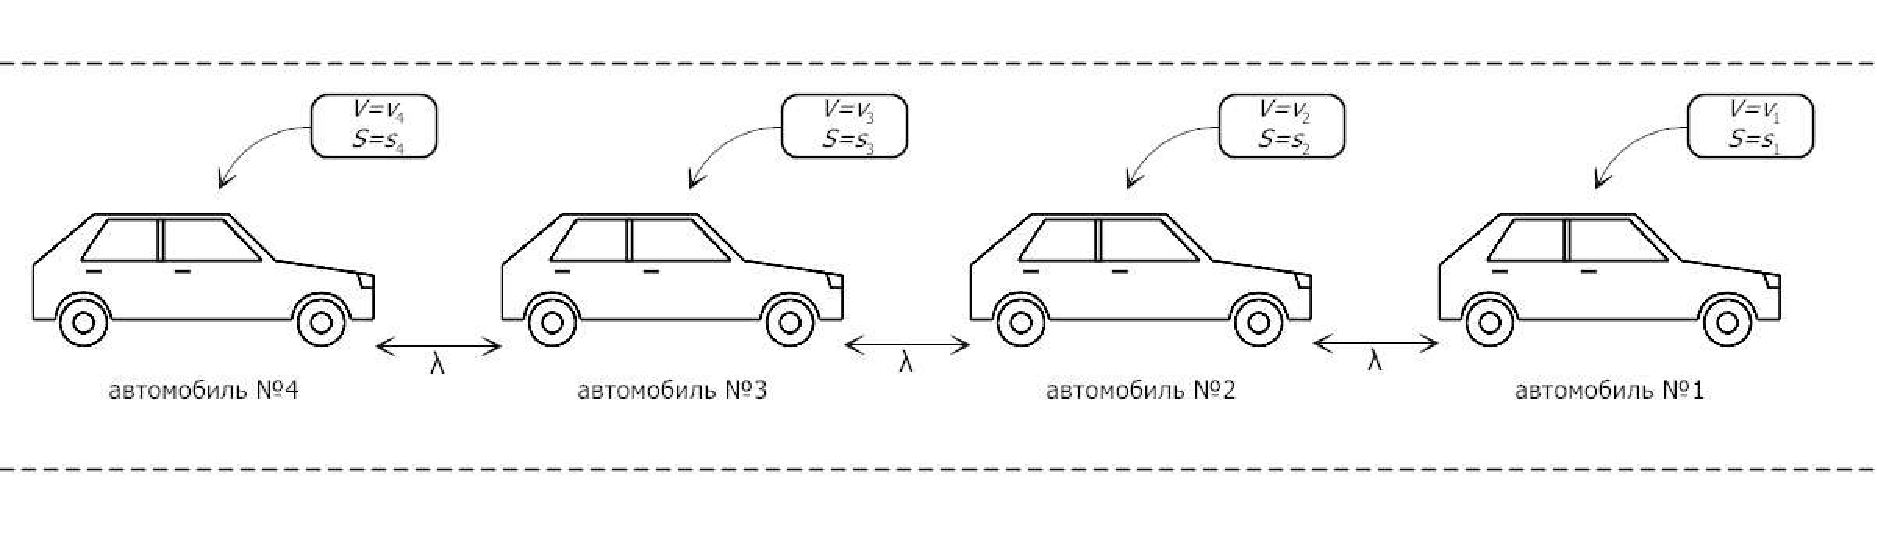
\includegraphics[keepaspectratio,width=160mm,height=70mm]{Images/car_following.pdf}
	\end{center}
	\caption{Автомобили, следующие друг за другом на безопасном расстоянии.}
	\label{car_following}
\end{figure}

Рассмотрим парадигму автомобиля, которая основана на очень простом правиле и уже довольно давно известна в литературе. Так как автомобили следуют друг за другом, преследователь всегда пытается максимизировать свою скорость с двумя ограничениями: ограничением ускорения и ограничением безопасности. Впервые данная парадигма была высказана ещё в 1975 \cite{GippsModel} и математически выглядит следующим образом:

\begin{equation*} \label{following_paradigm}
v_f(t) = \min(v_f^d(t), v_f^s(t)),
\end{equation*}
где $v_f(t)$ - скорость преследователя в момент времени $t$, $v_f^d(t)$ - максимальная возможная скорость с \textbf{ограничением ускорения} (demand speed), $v_f^s(t)$ - максимальная возможная скорость с \textbf{ограничением безопасности} (supply speed).

Под ограничением ускорения стоит понимать физические ограничения скорости и ускорения транспортного средства, а также условия комфорта, необходимые водителю. Эта величина описывает траекторию транспортного средства, которое свободно разгоняется до максимальной желаемой скорости при отсутствии впереди идущих транспортных средств. Ограничение безопасности - это то, как траектория транспортного средства зависит от впереди идущего транспортного средства (лидера).

\section{Обзор, анализ и модификация существующих математических моделей}
\subsection{Модель свободного движения}

Для начала рассмотрим простую ситуацию, когда на дороге есть всего одно транспортное средство. В качестве транспортного средства будем рассматривать материальную точку, что позволит не учитывать его внутреннюю структуру и внешние габариты. 

При движении одного транспортного средства по пустой дороге для него нет никаких ограничений за исключением его технических характеристик. В такой ситуации автомобиль разгонится до максимальной желаемой скорости и будет продолжать с ней движение. Такое поведение будем называть свободным движением. 

Для описания свободного движения можно использовать хорошо известное обыкновенное дифференциальное уравнение вида: 
\begin{equation} \label{free_drive}
\begin{cases}
\begin{split}
\ddot{x}&(t) = \alpha\left( 1-\left( \dfrac{\dot{x}(t)}{v_{max}}\right)^\delta \right) \\
&x(0)=x_0, \quad \dot{x}(0)=v_{0}
\end{split}
\end{cases}.
\end{equation}
В уравнении \eqref{free_drive} за $x$ обозначено положение транспортного средства, а за $\dot{x}$ и $\ddot{x}$ скорость и ускорение соответственно.

Из уравнения \eqref{free_drive} видно, что свободное движение характеризуется максимально желаемой (допустимой) скоростью $v_{max}$, начальной скоростью $v_{0}$, начальным положением транспортного средства $x_0$, максимальным ускорением $\alpha$ и показателем степени $\delta$, определяющим, как ускорение уменьшается с ростом скорости.

В уравнении \eqref{free_drive} вынесем знаменатель за скобку и будем считать полученное выражение за коэффициент ускорения $a=\dfrac{\alpha}{v_{max}^\delta}$. Таким образом, получаем следующую модель для свободного двигающегося автомобиля:

\begin{equation} \label{free_drive_with_initial_conditions}
\begin{cases}
\begin{split}
\ddot{x}&(t) = a\left( v_{max} - \dot{x}(t)\right)^\delta \\
&x(0)=x_0, \quad \dot{x}(0)=v_0
\end{split}
\end{cases}.
\end{equation}

Решения уравнения \eqref{free_drive_with_initial_conditions} имеют схожую динамику при различных значениях $\delta$. Это хорошо видно из рисунка \ref{free_drive_with_delta}, на котором изображены графики\footnote{Графики в данной работе выполнены с использованием системы компьютерной алгебры Wolfram Mathematica \cite{WolframMathematica}. Исходный код графиков находится на диске в приложение \ref{att2}.} решения уравнения \eqref{free_drive_with_initial_conditions} при разных $\delta$.

\begin{figure}[h!]
	\begin{center}
		\begin{minipage}[h!]{0.48\linewidth}
			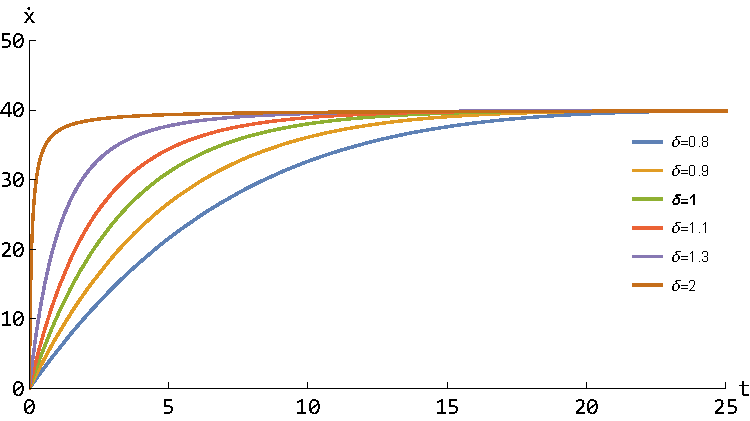
\includegraphics[width=1\linewidth,height=0.2\textheight]
			{Images/free_drive_speed_with_different_delta.pdf}
		\end{minipage}
		\caption{Графики изменения скорости при разных $\delta$ с параметрами: $a=0.15$, $v_{max}=40$, $x_0=0$, $v_0=0$.}
		\label{free_drive_with_delta}
	\end{center}
\end{figure}

Таким образом, без потери общности можно рассматривать модель \eqref{free_drive_with_initial_conditions} с коэффициентом $\delta=1$, что соответствует линейному уменьшению ускорения с ростом скорости.

Система \eqref{free_drive_with_initial_conditions} при $\delta=1$ имеет решение в явном виде:
\begin{equation*}
x(t) =\dfrac{1}{a}\left(av_{max}t+v_{max}e^{-at}-v_{max}-v_0e^{-at}+v_0+ax_0\right).
\end{equation*}
Из уравнения \eqref{free_drive_with_initial_conditions} видно, что при $v_0=v_{max}$ ускорения нет. Такое поведение согласуется с динамикой реального транспортного средства.

На рисунке \ref{free_drive_without_stop} изображены графики изменения скорости и расстояния для свободно двигающегося автомобиля.
\begin{figure}[h!]
	\begin{center}
		\begin{minipage}[h!]{0.48\linewidth}
			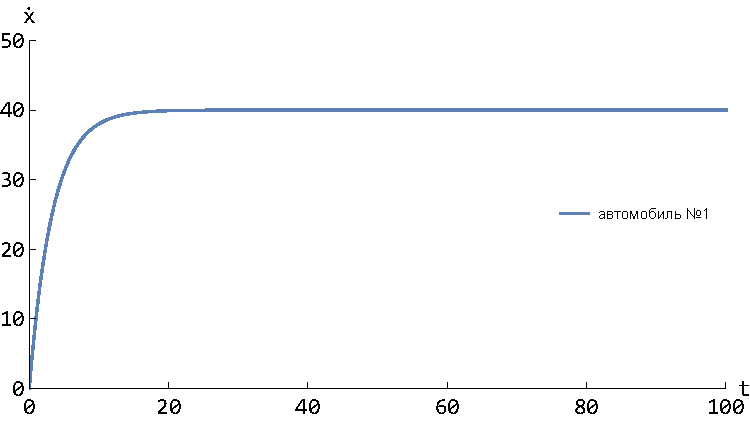
\includegraphics[width=1\linewidth,height=0.2\textheight]
			{Images/free_drive_speed.pdf}
		\end{minipage}
		\hfill 
		\begin{minipage}[h!]{0.48\linewidth}
			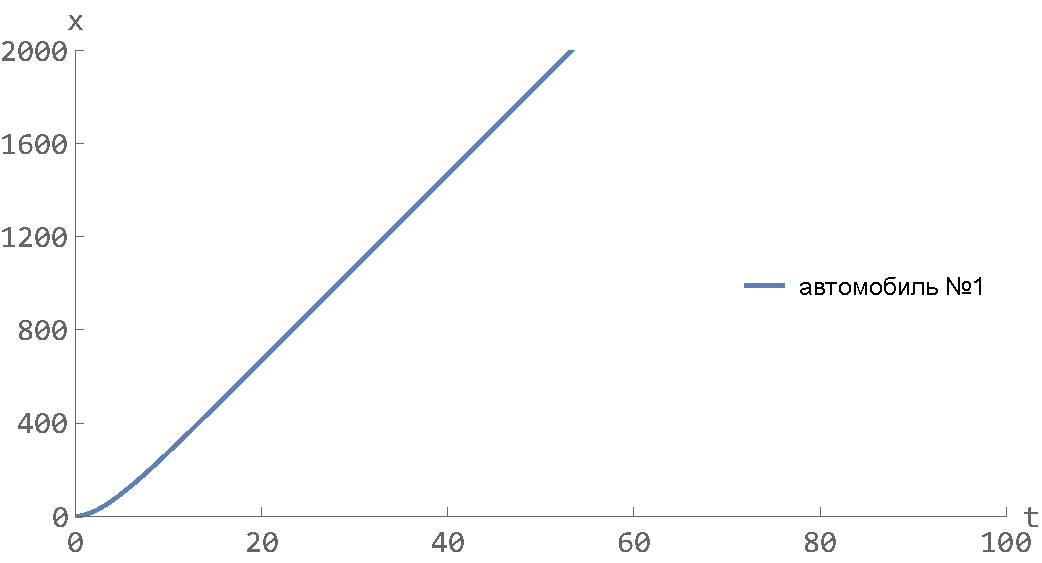
\includegraphics[width=1\linewidth,height=0.2\textheight]
			{Images/free_drive_distance.pdf}
		\end{minipage}
		\caption{Графики изменения скорости (слева) и расстояния (справа) для автомобиля при свободном движении без остановки с параметрами: $a=0.3$, $v_{max}=40$, $x_0=0$, $v_0=0$.}
		\label{free_drive_without_stop}
	\end{center}
\end{figure}

Из графиков видно, что автомобиль, разогнавшись до максимальной допустимой (желаемой) скорости, бесконечно двигается вперёд. Данная модель описывает момент старта автомобиля, его разгон и движение с постоянной скоростью. Под стартом автомобиля будем понимать момент начала разгона. В более жизненных ситуациях присутствуют процессы обратные разгону и старту - торможение и остановка.

Для описания остановки автомобиля рассмотрим дифференциальное уравнение, схожее с \eqref{free_drive_with_initial_conditions}: 
\begin{equation} \label{stop_drive_with_initial_conditions}
\begin{cases}
\begin{split}
\ddot{x}&(t) = q\left( v_{min} - \dot{x}(t)\right) \\
&x(0)=x_0, \quad \dot{x}(0)=v_0
\end{split}
\end{cases}.
\end{equation}
Из уравнения \eqref{stop_drive_with_initial_conditions} видно, что торможение характеризуется минимальной (желаемой) скоростью $v_{min}$, начальной скоростью $v_{0}$, начальным положением транспортного средства $x_0$ и коэффициентом торможения $q$. Под минимальной скоростью будем понимать такую скорость, до которой водитель транспортного средства хочет снизить свою текущую скорость. Это может быть и ненулевая величина, в некоторых случаях водитель не хочет останавливаться полностью, а хочет лишь снизить скорость до какого-то значения.

Система \eqref{stop_drive_with_initial_conditions} имеет решение в явном виде, аналогичное системе \eqref{free_drive_with_initial_conditions}:
\begin{equation*}
x(t) = \dfrac{1}{q}\left(qv_{min}t+v_{min}e^{-qt}-v_{min}-v_0e^{-qt}+v_0+qx_0\right).
\end{equation*}

Из уравнения \eqref{stop_drive_with_initial_conditions} видно, что при $v_0=v_{min}$ торможения нет. Данное поведение, аналогично случаю для ускорения, согласуется с динамикой реального транспортного средства.

Уравнения \eqref{free_drive_with_initial_conditions} и  \eqref{stop_drive_with_initial_conditions} описывают два разных вида движения. Для получения общей модели, описывающей оба этих вида движения, необходимо объединить их в одну. Предположим, что в нулевой момент времени происходит первая фаза движения - старт автомобиля и его разгон. Затем, с некоторого момента времени $t_s$ (stop time), происходит вторая фаза движения - автомобиль начинает тормозить. Введём две релейные функции $R_{a}(t)$ и $R_{b}(t)$, вида:  

\begin{equation*} 
R_{a}(t)=
\begin{cases}
\begin{split}
&1, \quad&\text{если } t<t_{s} \\
&0, \quad&\text{если } t\geq t_{s}
\end{split}
\end{cases},
\qquad
R_{b}(t)=
\begin{cases}
\begin{split}
&0, \quad&\text{если } t<t_{s} \\
&1, \quad&\text{если } t\geq t_{s}
\end{split}
\end{cases}.
\end{equation*}
Релейная функция $R_{a}(t)$ ``включается'', когда автомобиль находится в фазе разгона (acceleration phase) и ``выключается'', когда автомобиль переходит в фазу торможения (braking phase). Функция $R_{b}(t)$ наоборот - ``выключается'' в фазе разгона и ``включается'' в фазе торможения. Функцию $R_{a}(t)$ можно выразить через $R_{b}(t)$ следующим образом $R_{a}(t) = (1-R_{b}(t))$. Обозначим $R_{a}(t)$ как $R(t)$ и получим релейную функцию, которая объединяет два вида движения:

\begin{equation} \label{relay_function}
R(t)=
\begin{cases}
\begin{split}
&1, \quad&\text{если } t<t_{s} \\
&0, \quad&\text{если } t\geq t_{s}
\end{split}
\end{cases}.
\end{equation}

С помощью полученной релейной функции \eqref{relay_function} объединим модели \eqref{free_drive_with_initial_conditions} и  \eqref{stop_drive_with_initial_conditions} и получим полную модель свободного движения:
\begin{equation} \label{free_drive_model}
\begin{cases}
\begin{split}
\ddot{x}(t) = &R(t) \left[ a\left(v_{max}-\dot{x}(t) \right)\right] + (1-R(t)) \left[ q\left( v_{min} - \dot{x}(t)\right) \right]  \\
&x(0)=x_0, \quad \dot{x}(0)=v_{0}
\end{split}
\end{cases}.
\end{equation}

Уравнения \eqref{free_drive_with_initial_conditions} и  \eqref{stop_drive_with_initial_conditions} различаются лишь коэффициентами и целевой скоростью $v_{target}$, под которой будем понимать скорость к которой стремится автомобиль во время движения. В случае ускорения это $v_{max}$, а в случае торможения $v_{min}$. С учётом данных предположений объединённую модель \eqref{free_drive_model} можно переписать в более компактном виде:

\begin{equation} \label{free_drive_model_short}
\begin{cases}
\begin{split}
\ddot{x}(t) = &R_s(t) \left(v_{target}-\dot{x}(t) \right) \\
x(0)&=x_0, \quad \dot{x}(0)=v_{0}
\end{split}
\end{cases},
\end{equation}
где $R_s(t)$ - релейная функция вида:
\begin{equation*}
R_s(t)=
\begin{cases}
\begin{split}
&a, \quad&\text{если } t<t_{s} \\
&q, \quad&\text{если } t\geq t_{s}
\end{split}
\end{cases}.
\end{equation*}

Модель \eqref{free_drive_model_short} эквивалентна \eqref{free_drive_model}, но менее информативна, так как в модели \eqref{free_drive_model} фазы разгона и торможения выделены в отдельные слагаемые.

На рисунке \ref{free_drive_with_stop} изображены графики изменения скорости и расстояния для свободно двигающегося автомобиля с остановкой по модели \eqref{free_drive_model}.

\begin{figure}[h!]
	\begin{center}
		\begin{minipage}[h!]{0.48\linewidth}
			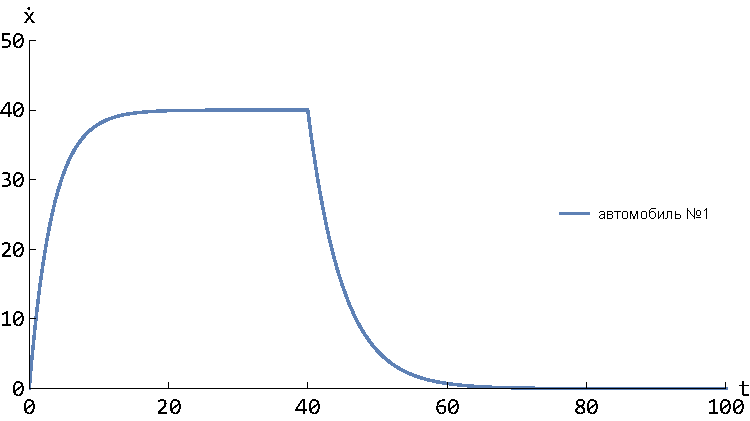
\includegraphics[width=1\linewidth,height=0.2\textheight]
			{Images/free_drive_speed_with_stop.pdf}
		\end{minipage}
		\hfill 
		\begin{minipage}[h!]{0.48\linewidth}
			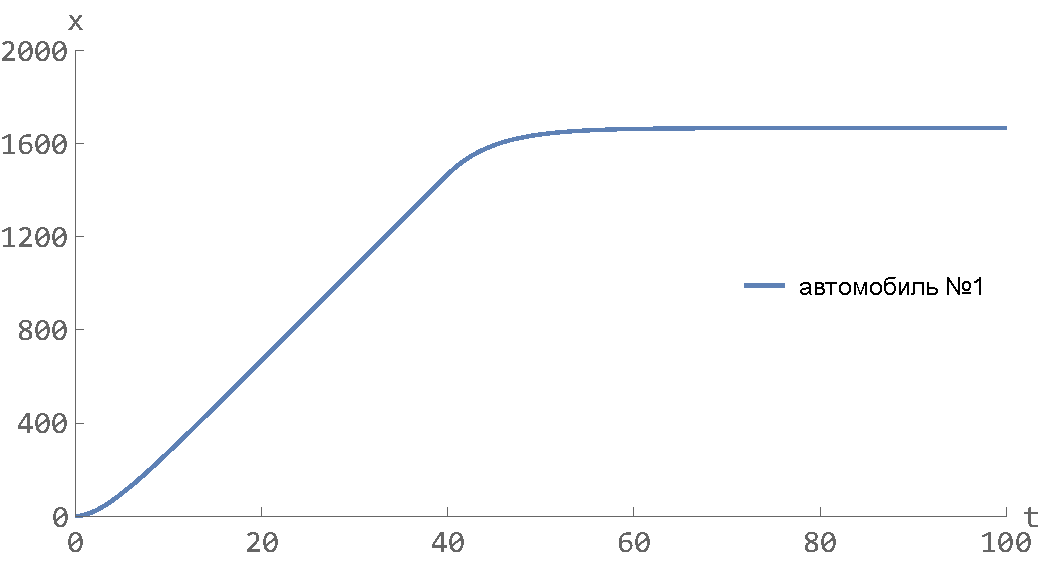
\includegraphics[width=1\linewidth,height=0.2\textheight]
			{Images/free_drive_distance_with_stop.pdf}
		\end{minipage}
		\caption{Графики изменения скорости (слева) и расстояния (справа) для автомобиля при свободном движении c остановкой с параметрами: $a=0.3$, $q=0.2$, $v_{max}=40$, $v_{min}=0$, $t_s=40$, $x_0=0$, $v_0=0$.}
		\label{free_drive_with_stop}
	\end{center}
\end{figure}

Из графиков видно, что автомобиль, разогнавшись до максимальной допустимой (желаемой) скорости, двигается с ней до наступления времени торможения. В этот момент автомобиль начинает тормозить и снижает свою скорость до минимальной желаемой и продолжает с ней движение или же, если минимальная скорость равна нулю ($v_{min}=0$), как на графиках \ref{free_drive_with_stop}, останавливается.
 
Таким образом, была получена модель \eqref{free_drive_model}, которая описывает все значимые фазы движения одного автомобиля, а именно разгон, само движение и торможение. Даная модель не учитывает внешних факторов, которые оказывают влияние на движение автомобиля, она зависит лишь от технических характеристик транспортного средства и от комфорта самого водителя. Эта модель подходит для описания динамики первого автомобиля в потоке. На остальные автомобили большое влияние оказывают впереди идущие транспортные средства, поэтому они вынуждены двигаться, подстраиваясь под движение лидера.

\subsection{``Простая'' модель следования за лидером}

Рассмотрим несколько автомобилей и занумеруем их индексом $n \in \mathbb{N}$ в соответствии с их порядковым номером на дороге. Предполагается, что ускорение $n$-ого автомобиля определяется состоянием соседних автомобилей, а именно наибольшее влияние оказывает непосредственно впереди идущий автомобиль (лидер).

Первая модель, основанная на принципе следования за лидером была разработана в 50-х годах прошлого века и предполагала, что каждый водитель адаптирует свою скорость к скорости лидирующего автомобиля:

\begin{equation} \label{follow_the_leader_first_model}
\ddot{x}_n(t) = \dfrac{1}{\gamma} (\dot{x}_{n-1}(t) - \dot{x}_{n}(t)), 
\end{equation}
где $\gamma$ - время адаптации водителя.

Данное уравнение было получено в работе Пайпса (Pipes) \cite{FirstFollowTheLeaderModel}. Модель, построенная на основе данного уравнения, является простой и плохо описывает свойства реального транспортного потока \cite{Shvetsov}.

В работе \cite{RefineFirstFollowTheLeaderModel} была предложена модификация уравнения \eqref{follow_the_leader_first_model}. В левую часть уравнения была введена задержка аргумента по времени $\tau$, которая отражает время реакции водителей на изменение скорости лидирующего автомобиля:

\begin{equation*}
\ddot{x}_n(t+\tau) = \dfrac{1}{\gamma} (\dot{x}_{n-1}(t) - \dot{x}_{n}(t)).
\end{equation*}
Произведя замену времени получим следующие уравнение:
\begin{equation} \label{follow_the_leader_with_two_delay}
\ddot{x}_n(t) = \dfrac{1}{\gamma} (\dot{x}_{n-1}(t-\tau) - \dot{x}_{n}(t-\tau)).
\end{equation}

Уравнение \eqref{follow_the_leader_with_two_delay} содержит запаздывание в двух слагаемых в правой части, то есть ускорение автомобиля зависит от разности скоростей, которые были у текущего и впереди идущего автомобилей $\tau$ времени назад.

Упростим уравнение \eqref{follow_the_leader_with_two_delay}, оставив в правой части запаздывание только у первого слагаемого, таким образом, ускорение автомобиля будет зависеть от его текущей скорости и скорости впереди идущего автомобиля $\tau$ времени назад. Множитель $\dfrac{1}{\gamma}$ будем интерпретировать как коэффициент мощности $d$, характеризующий мощность двигателя автомобиля. С учётом проведённых модификаций уравнение примет вид:

\begin{equation} \label{follow_the_leader_with_delay}
\ddot{x}_n(t) = d_{n} (\dot{x}_{n-1}(t-\tau) - \dot{x}_{n}(t)).
\end{equation}

Без потери общности будем считать, что все автомобили имеют одинаковые технические характеристики $d_n = d$, а все водители одинаково оценивают дорожную ситуацию и реагируют на её изменения с одинаковой скоростью.

Уравнение \eqref{follow_the_leader_with_delay} можно проинтегрировать и рассматривать модель, зависящую от положения самого транспортного средства и положения лидера. Данный подход подробно описан в \cite{Course}. В данной работе будем рассматривать уравнение в исходном виде. 

Уравнение \eqref{follow_the_leader_with_delay} не описывает движение первого автомобиля, поэтому дополним его ранее полученным уравнением свободного движения. Таким образом, динамика первого автомобиля будет описываться \eqref{free_drive_model}, а остальные автомобили будут двигаться согласно разностному уравнению \eqref{follow_the_leader_with_delay}. Будем считать, что в начальный момент времени все автомобили находятся на одинаковом расстоянии $\lambda$ друг от друга. Математически это выглядит следующим образом:

\begin{equation} \label{follow_the_leader_full_model}
\begin{cases}
\begin{split}
\ddot{x}_1(t)& = R(t) \left[ a\left(v_{max}-\dot{x}_1(t) \right)\right] + (1-R(t)) \left[ q\left( v_{min} - \dot{x}_1(t)\right) \right] \\
&x_{1}(0)=x_0, \quad \dot{x}_{1}(0)=v_{0}\\
\ddot{x}_{n}(t)& = d(\dot{x}_{n-1}(t-\tau)-\dot{x}_{n}(t)) \\
&x_n(t)=x_0-(n-1)\lambda, \quad \dot{x}_n(t)=v_{n}, \quad \text{при } t \in [-\tau,0] \text{ и } n\geq2
\end{split}
\end{cases}.
\end{equation}

На рисунке \ref{follow_the_leader} изображены графики изменения скорости и расстояния для нескольких автомобилей, движущихся согласно модели \eqref{follow_the_leader_full_model}.

\begin{figure}[h!]
	\begin{center}
		\begin{minipage}[h!]{0.48\linewidth}
			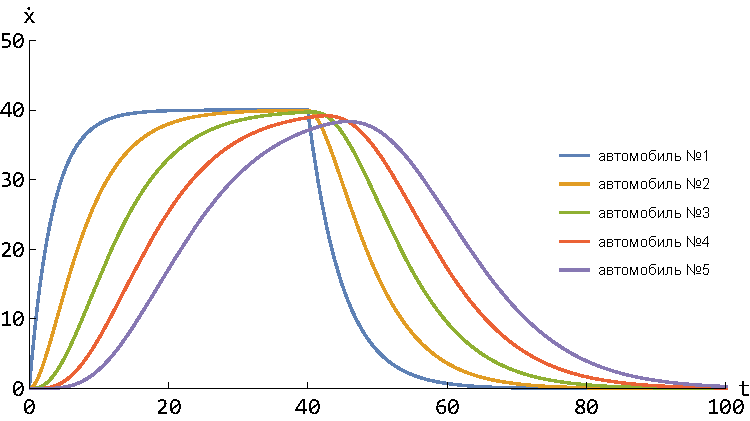
\includegraphics[width=1\linewidth,height=0.2\textheight]
			{Images/simple_model_speed.pdf}
		\end{minipage}
		\hfill 
		\begin{minipage}[h!]{0.48\linewidth}
			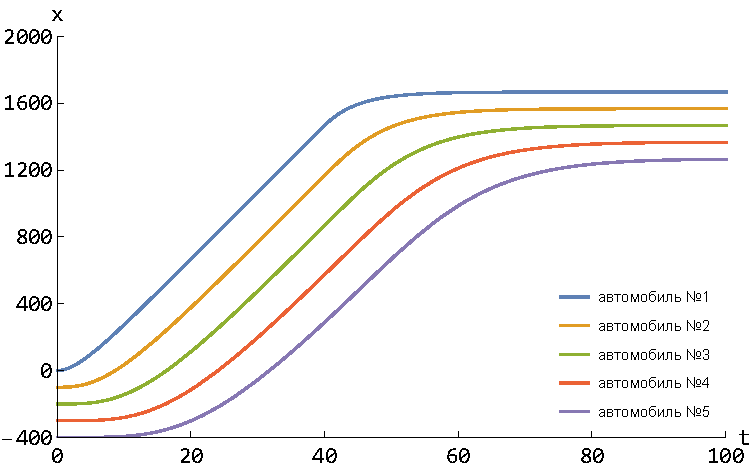
\includegraphics[width=1\linewidth,height=0.2\textheight]
			{Images/simple_model_distance.pdf}
		\end{minipage}
		\caption{Графики изменения скорости (слева) и расстояния (справа) для транспортного потока с остановкой с параметрами: $\tau=1$, $a=0.3$, $q=0.2$, $v_{max}=40$, $v_{min}=0$, $\lambda=100$, $d=0.2$, $t_s=40$, $x_0=0$, $v_n=0$, $v_0=0$.}
		\label{follow_the_leader}
	\end{center}
\end{figure}

Из графиков видно, что автомобили разгоняются до максимальной желаемой скорости и двигаются до момента времени $t_s$, начиная с которого, первый автомобиль тормозит и останавливается. Остальные автомобили, повторяя динамику первого автомобиля, также останавливаются. Все движение происходит с сохранением безопасной дистанции между автомобилями, что соответствует реальному транспортному потоку, так как сокращение безопасного расстояния подразумевает появление аварийной ситуации.

Результаты исследования модели \eqref{follow_the_leader_full_model} совпадают с  результатами исследований моделей \eqref{follow_the_leader_with_two_delay} и проинтегрированной \eqref{follow_the_leader_full_model} из работ \cite{RefineFirstFollowTheLeaderModel} и \cite{Course} соответственно. С помощью регулировки коэффициентов в моделях можно добиться полной идентичности решений. Данные модели не учитывают расстояния между транспортными средствами, имеют сравнительно простую динамику, и могут быть в равной мере использованы для моделирования движения транспортных потоков. 

\subsection{Модель следования за лидером ``Дженерал моторс''}

Группа инженеров из компании ``Дженерал моторс'' (General Motors) в своей работе \cite{GazisModel} предложила дополнительную модификацию для уравнения  \eqref{follow_the_leader_with_two_delay}. Основой этой модификации является идея рассмотреть вместо постоянного коэффициента $\dfrac{1}{\gamma}$ динамическую величину $S(t)$, которую можно интерпретировать как коэффициент чувствительности. 

Коэффициент чувствительности $S(t)$ характеризует скорость реакции водителя к изменению скорости лидера и зависит от его текущей скорости водителя и расстояния до лидера. Чувствительность возрастает при уменьшении дистанции до лидера, таким образом, коэффициент $S(t)$ можно представить в виде:

\begin{equation} \label{gazis_coefficient}
S(t) = \dfrac{\eta_{l,m}\dot{x}_n^{m_1}(t)}{(x_{n-1}(t-\tau)-x_n(t-\tau))^{m_2}},
\end{equation}
где $\eta$ - константа, характеризующая движение, а $m_1$ и $m_2$ - эмпирически подбираемые константы, также характеризующие движение. Коэффициент чувствительности был получен в работе Газиса, Хермана и Ротери (Gazis-Herman-Rothery, GHR)  \cite{GazisModel}. Модель, полученная с учётом этого коэффициента выглядит следующим образом:   
\begin{equation} \label{gazis_model}
\ddot{x}_n(t) = \dfrac{\eta_{l,m}\dot{x}_n^{m_1}(t)}{(x_{n-1}(t-\tau)-x_n(t-\tau))^{m_2}} (\dot{x}_{n-1}(t-\tau) - \dot{x}_{n}(t-\tau)).
\end{equation}

Изучение модели, полученной Газисом-Херманом-Ротери, в исходном виде описано в работах \cite{StudyingGazisModel_1},  \cite{StudyingGazisModel_2} и  \cite{StudyingGazisModel_3}. При значениях параметров $m_1 \approx 0.8$, $m_2 \approx 2.8$ \cite{StudyingGazisModel_1} или $m_1 = 0.953$, $m_2 = 3.05$ \cite{StudyingGazisModel_2}, \cite{StudyingGazisModel_3} получаются результаты наиболее схожие с реальными данными.

Аналогично ``простой'' модели, данная модель \eqref{gazis_model} плохо описывать движение первого автомобиля, поэтому дополним её уравнением \eqref{free_drive_model} и рассмотрим полученную модель движения транспортного потока:

\begin{equation} \label{full_gazis_model}
\begin{cases}
\begin{split}
\ddot{x}_1(t)& = R(t) \left[ a\left(v_{max}-\dot{x}_1(t) \right)\right] + (1-R(t)) \left[ q\left( v_{min} - \dot{x}_1(t)\right) \right] \\
&x_{1}(0)=x_0, \quad \dot{x}_{1}(0)=v_{0}\\
\ddot{x}_n(t)& = \dfrac{\eta_{l,m}\dot{x}_n^{m_1}(t)}{(x_{n-1}(t-\tau)-x_n(t-\tau))^{m_2}} (\dot{x}_{n-1}(t-\tau) - \dot{x}_{n}(t-\tau)) \\
&x_n(t)=x_0-(n-1)\lambda, \quad \dot{x}_n(t)=v_{n}, \quad \text{при } t \in [-\tau,0] \text{ и } n\geq2
\end{split}
\end{cases}.
\end{equation}

Полученные модели \eqref{gazis_model} и \eqref{full_gazis_model} очень сильно зависят от эмпирически подбираемых констант $m_1$ и $m_2$. При их неудачном выборе решения не согласуются с реальными данными. На рисунках \ref{gazis_model_good} и \ref{gazis_model_bad} изображены графики решений для ``удачного'' и ``неудачного'' выбора параметров. 
\begin{figure}[h!]
	\begin{center}
		\begin{minipage}[h!]{0.48\linewidth}
			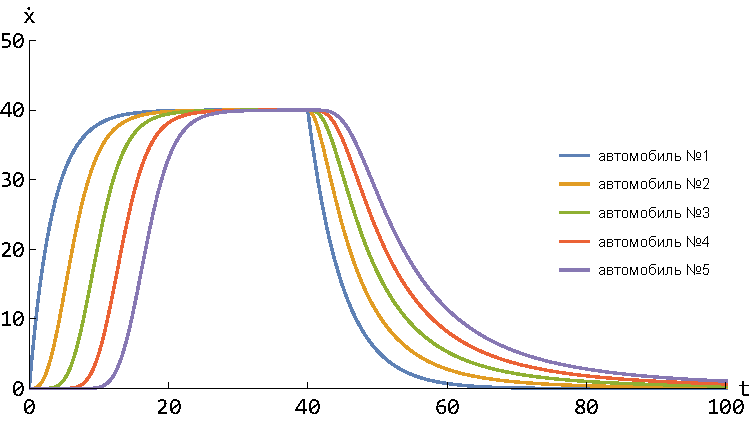
\includegraphics[width=1\linewidth,height=0.2\textheight]
			{Images/gazis_model_good_speed.pdf}
		\end{minipage}
		\hfill 
		\begin{minipage}[h!]{0.48\linewidth}
			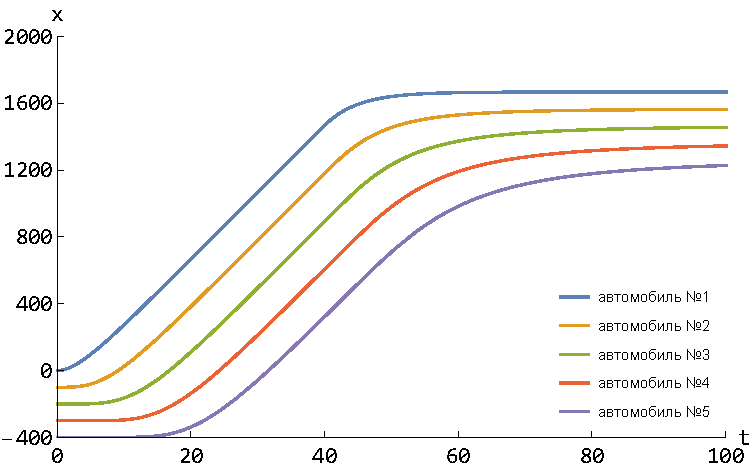
\includegraphics[width=1\linewidth,height=0.2\textheight]
			{Images/gazis_model_good_distance.pdf}
		\end{minipage}
		\caption{Графики изменения скорости (слева) и расстояния (справа) для модели Газиса-Хермана-Ротери с ``удачным'' выбором параметров: $\tau=1$, $a=0.3$, $q=0.2$, $v_{max}=40$, $v_{min}=0$, $\lambda=100$, $t_s=40$, $x_0=0$, $v_0=0$, $\eta=0.4$, $\boldsymbol{m_1=0.4}$, $\boldsymbol{m_2=0.3}$}
		\label{gazis_model_good}
	\end{center}
\end{figure}

\begin{figure}[h!]
	\begin{center}
		\begin{minipage}[h!]{0.48\linewidth}
			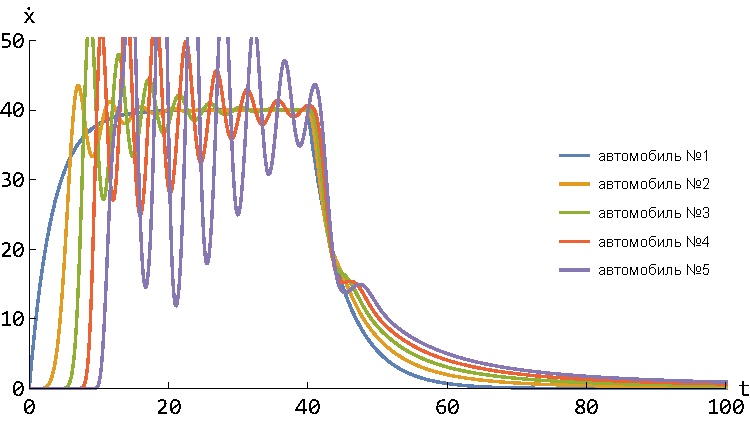
\includegraphics[width=1\linewidth,height=0.2\textheight]
			{Images/gazis_model_bad_speed.pdf}
		\end{minipage}
		\hfill 
		\begin{minipage}[h!]{0.48\linewidth}
			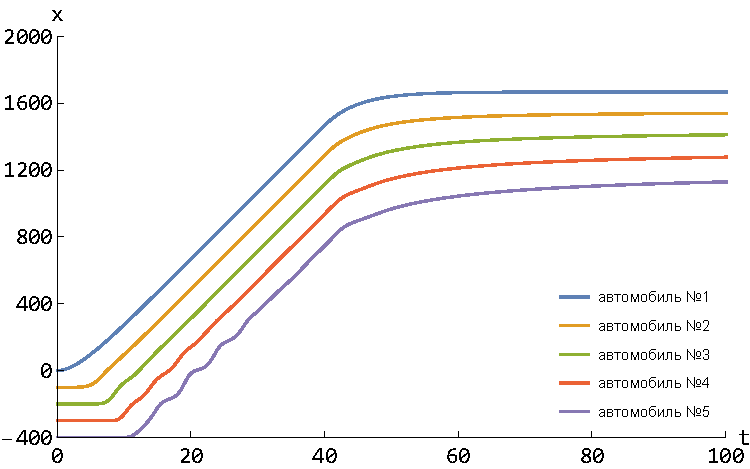
\includegraphics[width=1\linewidth,height=0.2\textheight]
			{Images/gazis_model_bad_distance.pdf}
		\end{minipage}
		\caption{Графики изменения скорости (слева) и расстояния (справа) для модели Газиса-Хермана-Ротери с ``неудачным'' выбором параметров: $\tau=1$, $a=0.3$, $q=0.2$, $v_{max}=40$, $v_{min}=0$, $\lambda=100$, $t_s=40$, $x_0=0$, $v_0=0$, $v_n=0$, $v_n=0$, $\eta=0.4$, $\boldsymbol{m_1=0.7}$, $\boldsymbol{m_2=0.3}$}
		\label{gazis_model_bad}
	\end{center}
\end{figure}

Графики на рисунке \ref{gazis_model_good} демонстрируют хорошую ситуацию, когда решения согласуются с реальным поведением транспортных средств на дороге. Графики же на рисунке \ref{gazis_model_bad} показывают плохую ситуацию. Скорость некоторых автомобилей с некоторого момента времени начинает сильно колебаться с большой амплитудой и не только превышает допустимую скорость, но и, в некоторых случая,х падает почти до нуля. Такое поведение невозможно в реальной жизни.

Из результатов исследования можно сделать вывод, что ни данная модель в исходном виде \eqref{gazis_model}, ни данная модель, дополненная уравнением движения первого автомобиля \eqref{full_gazis_model} не подходят для моделирования транспортного потока. Большая зависимость от правильного выбора параметров $m_1$ и $m_2$, а также несвязанность этих параметров с реальными физическими величинами усложняет моделирование и не гарантирует получение правильной динамики движения транспортных потоков. 

\subsection{Модель ``разумного водителя''}
В настоящее время наиболее современной и популярной моделью движения транспортных потоков является модель ``разумного водителя'' (Intelligent Driver Model, IDM), разработанная Трайбером (Treiber) с соавторами \cite{TreiberModel_1}, \cite{TreiberModel_2} в конце прошлого начале нынешнего века. 

В модели ``разумного водителя'' ускорение автомобиля зависит от текущей скорости самого автомобиля, от скорости впереди идущего автомобиля и расстояния между ними. Математически это можно записать в следующем виде:
\begin{equation*}
\ddot{x}_n(t)=f(t, \dot{x}_n,\dot{x}_{n-1}, x_{n-1}-x_n).
\end{equation*} 

В модели ``разумного водителя'' движение автомобиля состоит из двух фаз. Первая фаза - это фаза разгона, в которой автомобиль пытается разогнаться до максимальной допустимой скорости. Вторая фаза - фаза торможения, в которой автомобиль замедляется, чтобы держаться на безопасном расстоянии от впереди идущей машины. Объединяя эти фазы получаем следующую модель:
\begin{equation} \label{treiber_model}
\ddot{x}_n(t)= \alpha\left( 1-\left( \dfrac{\dot{x}_n(t)}{v_{max}}\right)^\delta \right) - \alpha\left( \dfrac{s^*_n(\dot{x}_n(t),\Delta \dot{x}_n(t))}{s_n}\right)^2,
\end{equation}
где $s_n$ - фактическое расстояние между автомобилями, а $s^*_n$ - желаемое.

Фактическое расстояние $s_n$ определяется разницей между положениями двух соседних автомобилей $s_n=x_{n-1}(t)-x_n(t)$. Желаемое расстояние  $s^*_n$ определяется формулой:
\begin{equation*}
s^*_n = \sigma_0+\sigma_1\sqrt{\dfrac{ \dot{x}_n(t)}{v_{max}}} +T \dot{x}_n(t)+ \dfrac{ \dot{x}_n(t)\Delta \dot{x}_n(t) }{2\sqrt{ab}},
\end{equation*}
где $\Delta \dot{x}_n(t) = \dot{x}_n(t)- \dot{x}_{n-1}(t)$ - разница скоростей автомобилей, $\sigma_0$ - расстояние между автомобилями, $\sigma_1$ - коэффициент регулировки скорости в заторе, $T$ - безопасный временной интервал, $b$ - коэффициент ``комфортного'' (не экстренного) торможения.

Можно заметить, что в модели \eqref{treiber_model} первое слагаемое - это модель свободного движения в исходном виде \eqref{free_drive}, а второе - это усовершенствованный коэффициент чувствительности \eqref{gazis_coefficient} из модели Газиса-Хермана-Ротери. Таким образом, можно сделать вывод, что в модели ``разумного водителя'' объединяются лучшие идеи ранее рассмотренных моделей.

Аналогично модели свободного движения рассмотрим модель ``разумного водителя'' \eqref{treiber_model} при линейном уменьшении ускорения с ростом скорости, то есть при $\delta=1$:

\begin{equation} \label{full_treiber_model}
\ddot{x}_n(t)= \alpha\bigg(\dfrac{v_{max}-\dot{x}_n(t)}{v_{max}} \bigg) - \alpha\bigg( \dfrac{\sigma_0+\sigma_1\sqrt{\frac{ \dot{x}_n(t)}{v_{max}}} +T \dot{x}_n(t)+ \frac{ \dot{x}_n(t)\Delta \dot{x}_n(t) }{2\sqrt{ab}}}{x_{n-1}(t)-x_n(t)}\bigg)^2.
\end{equation}

Аналогично двум предыдущим случаям данная модель \eqref{full_treiber_model} плохо описывает динамику первого автомобиля, поэтому дополним её уравнением \eqref{free_drive_model} и рассмотрим полученную модель движения транспортного потока:
\begin{equation} \label{full_treiber_model_with_first_car} 
\begin{cases}
\begin{split}
\ddot{x}_1(t)& = R(t) \left[ a\left(v_{max}-\dot{x}_1(t) \right)\right] + (1-R(t)) \left[ q\left( v_{min} - \dot{x}_1(t)\right) \right] \\
&x_{1}(0)=x_0, \quad \dot{x}_{1}(0)=v_{0}\\
\ddot{x}_n(t)& = \alpha\bigg(\dfrac{v_{max}-\dot{x}_n(t)}{v_{max}} \bigg) - \alpha\bigg( \dfrac{\sigma_0+\sigma_1\sqrt{\frac{ \dot{x}_n(t)}{v_{max}}} +T \dot{x}_n(t)+ \frac{ \dot{x}_n(t)\Delta \dot{x}_n(t) }{2\sqrt{ab}}}{x_{n-1}(t)-x_n(t)}\bigg)^2 \\
&x_n(t)=x_0-(n-1)\lambda, \quad \dot{x}_n(t)=v_{n}, \quad \text{при } t \in [-\tau,0] \text{ и } n\geq2
\end{split}
\end{cases}.
\end{equation}

На рисунке \ref{treiber_model_img} изображены графики изменения скорости и расстояния для нескольких автомобилей, движущихся друг за другом, согласно модели \eqref{full_treiber_model_with_first_car}.

\begin{figure}[h!]
	\begin{center}
		\begin{minipage}[h!]{0.48\linewidth}
			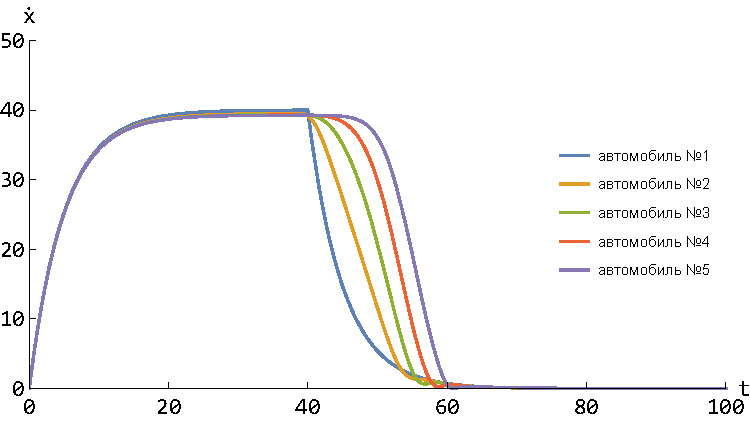
\includegraphics[width=1\linewidth,height=0.2\textheight]
			{Images/treiber_model_speed.pdf}
		\end{minipage}
		\hfill 
		\begin{minipage}[h!]{0.48\linewidth}
			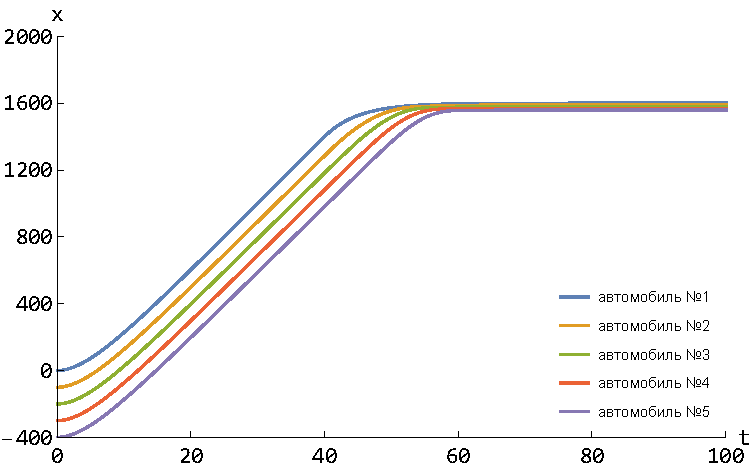
\includegraphics[width=1\linewidth,height=0.2\textheight]
			{Images/treiber_model_distance.pdf}
		\end{minipage}
		\caption{Графики изменения скорости (слева) и расстояния (справа) для модели ``разумного водителя'' с параметрами: $a=0.2$, $\alpha=8$, $q=0.2$, $v_{max}=40$, $v_{min}=0$, $\lambda=100$, $t_s=40$, $x_0=0$, $v_0=0$, $v_n=0$, $\sigma_0=10$,$\sigma_1=5$, $T=0.1$, $b=2$ }
		\label{treiber_model_img}
	\end{center}
\end{figure}

На графиках \ref{treiber_model_img} видна некорректная динамика. Так из графика скорости видно, что автомобили начинают движение одновременно и не достигают максимальной возможной скорости, так как скорости автомобилей отделены друг от друга на некоторую величину. Также из графиков видно, что при остановке скорость автомобиля начинает колебаться, в то время как автомобили подъезжают вплотную друг к другу и между ними не остаётся безопасного расстояния. Такое поведение не соответствует динамике движения реального транспортного потока. 

Таким образом, модель ``разумного водителя'' в исходном виде не подходит для моделирования динамики транспортных потоков. Некорректная динамика и большое количества параметров делают модель непригодной для использования.

Улучшить модель ``разумного водителя'' можно путём сокращения количества параметров. Так, например, параметры $\sigma_1$ (коэффициент регулировки скорости в заторе) и $T$ (безопасный временной интервал) имеют неясную содержательную интерпретацию и могут быть приравнены к нулю. Данная модификация упрощает модель, но не меняет её динамику, тем самым сохраняя несоответствие реальным данным.

\section{Построение новой математической модели}
Рассмотренные ранее модели обладают рядом недостатков и могут быть лишь частично использованы для моделирования транспортных потоков. 

Используя опыт и некоторые идеи ранее рассмотренных модель, построим новую модель, которая будет описывать движение $n \in \mathbb{N}$ автомобилей. Аналогично предыдущим моделям обозначим за $x$ положение транспортного средства, а за $\dot{x}$ и $\ddot{x}$ их скорость и ускорение соответственно. Все автомобили будем считать материальными точками и не будем учитывать их внутреннюю структуру и внешние габариты.

Все движение автомобиля разделим на две фазы: ускорение и торможение, причём в конкретный момент времени автомобиль либо разгоняется, либо тормозит. Для этого введём релейную функцию вида:

\begin{equation*}
R(\Delta x_{n}(t,\tau))=
\begin{cases}
\begin{split}
&1,\quad &\text{если }\Delta x_{n}(t,\tau) >S \\
&0,\quad &\text{если }\Delta x_{n}(t,\tau) \leq S
\end{split}
\end{cases},
\end{equation*}
где $\tau$ - время реакции водителя, $\Delta x_{n}(t,\tau)=x_{n-1}(t-\tau)-x_n(t)$ - расстояние между соседними автомобилями, а $S$ - тормозной путь. Под \textbf{тормозным путём} будем понимать расстояние, которое проходит транспортное средство с момента срабатывания тормозной системы до полной остановки \cite{PDD}. Для расчёта данной величины воспользуемся хорошо известной формулой \cite{Physics}:
\begin{equation*} 
S=\dfrac{v^2}{2\mu g},
\end{equation*}
где $v$ - текущая скорость транспортного средства, $\mu$ - коэффициент трения, $g$ - ускорение свободного падения. Из определения тормозного пути следует, что автомобиль остановится вплотную к впереди идущему автомобилю, в случае его моментальной остановки. Для того чтобы разделить автомобили, к тормозному пути прибавим константу $c > 0$. В качестве её возьмём единицу расстояния и получим $S+1$. Таким образом, получаем реле, которое будет переключать фазы движения автомобиля:
\begin{equation}\label{rele}
R(\Delta x_{n}(t,\tau))=
\begin{cases}
\begin{split}
&1,\quad &\text{если }\Delta x_{n}(t,\tau) > \dfrac{\dot{x}_n^2(t)}{2\mu g}+1 \\
&0,\quad &\text{если }\Delta x_{n}(t,\tau) \leq \dfrac{\dot{x}_n^2(t)}{2\mu g}+1
\end{split}
\end{cases}.
\end{equation}

Первая фаза движения - это разгон. Для описания разгона воспользуемся принципом, при котором преследующий автомобиль подстраивает свою скоростью относительно впереди идущего:

\begin{equation*}
\ddot{x}_n(t)= \bigg[ a(\dot{x}_{n-1}(t-\tau)-\dot{x}_n(t))\bigg],
\end{equation*}
где $a$ - коэффициент ускорения.

Вторая фаза движения - это торможение. Торможение автомобиля зависит от разности расстояний и скоростей между самим автомобилем и впереди идущим автомобилем, а также от безопасной дистанции между ними. Математически это можно записать следующим образом: 

\begin{equation*}
\ddot{x}_n(t)= \left[  q\left(  \dfrac{\dot{x}_n^2(t)\left[  \dot{x}_{n-1}(t-\tau) - \dot{x}_n(t) \right]}{(x_{n-1}(t-\tau)-x_n(t)-l)^2}\right) \right],
\end{equation*}
где $l$ - безопасное расстояние между автомобилями, a $q$ - коэффициент торможения.

Таким образом, объединяя обе фазы, получаем новую математическую модель движения транспортных потоков:
\begin{equation} \label{my_model} 
\begin{split}
\ddot{x}_n(t)= &R(\Delta x_n(t,\tau))\bigg[ a(\dot{x}_{n-1}(t-\tau)-\dot{x}_n(t))\bigg]  +\\+& (1-R(\Delta x_n(t,\tau)))\left[  q\left(  \dfrac{\dot{x}_n^2(t)\left[  \dot{x}_{n-1}(t-\tau) - \dot{x}_n(t) \right]}{(x_{n-1}(t-\tau)-x_n(t)-l)^2}\right) \right] 
\end{split}.
\end{equation}

Данная разностная модель описывает все автомобили потока. Для описания первого автомобиля модель необходимо дополнить начальными данными. Таким образом, для первого автомобиля (при $n=1$) доопределим значения $x_{0}$ и $\dot{x}_{0}$. За $x_{0}$ будем считать расстояние, которое должен проехать автомобиль, например, это может быть расстояние до светофора или иного препятствия $x_{0}=L$. За $\dot{x}_{0}$ в первом слагаемом будем считать максимальную желаемую скорость $\dot{x}_{0}=v_{max}$, а во втором минимальную желаемую скорость, то есть скорость до которой нужно оттормозиться $\dot{x}_{0}=v_{min}$.

Будем считать, что в начальный момент времени первый автомобиль находится в положении $\lambda_0$, и между соседними автомобилями расстояние $\lambda$. Таким образом, место положение каждого автомобиля можно определить выражением $\lambda_0-(n-1)\lambda$. Также будем считать, что начальное расстояние между соседними автомобилями $\lambda$ строго больше чем безопасное расстояние $l$, что соответствует неравенству $\lambda > l$.

Добавив начальные условия к модели \eqref{my_model} получим полную математическую модель движения транспортных потоков:

\begin{equation} \label{new_model} 
\begin{cases}
\begin{split}
\ddot{x}_n(t)= &R(\Delta x_n(t,\tau))\bigg[ a(\dot{x}_{n-1}(t-\tau)-\dot{x}_n(t))\bigg]  +\\+& (1-R(\Delta x_n(t,\tau)))\left[  q\left(  \dfrac{\dot{x}_n^2(t)\left[  \dot{x}_{n-1}(t-\tau) - \dot{x}_n(t) \right]}{(x_{n-1}(t-\tau)-x_n(t)-l)^2}\right) \right] \\
 \quad x_n(t)&=\lambda_0-(n-1)\lambda, \quad \dot{x}_n(t)=v_{n}, \quad \text{при } t \in [-\tau,0] \text{ и } n\geq2
\end{split}
\end{cases}.
\end{equation}

На рисунке \ref{new_model_picture} изображены графики изменения скорости и расстояния для нескольких автомобилей, двигающихся согласно модели \eqref{new_model}.

\begin{figure}[h!]
	\begin{center}
		\begin{minipage}[h!]{0.48\linewidth}
			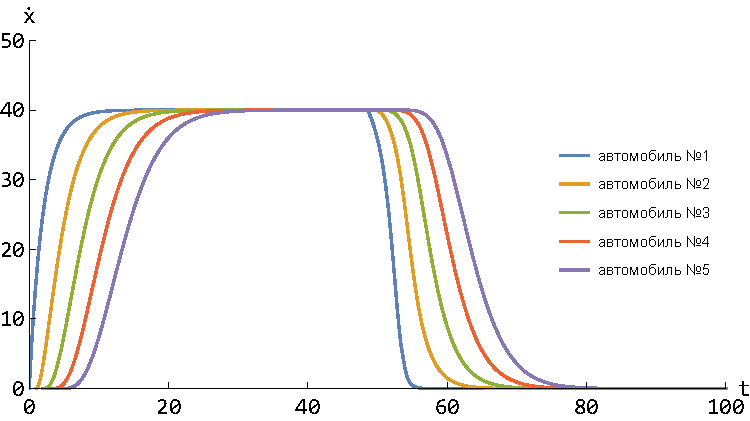
\includegraphics[width=1\linewidth,height=0.2\textheight]
			{Images/new_model_speed.pdf}
		\end{minipage}
		\hfill 
		\begin{minipage}[h!]{0.48\linewidth}
			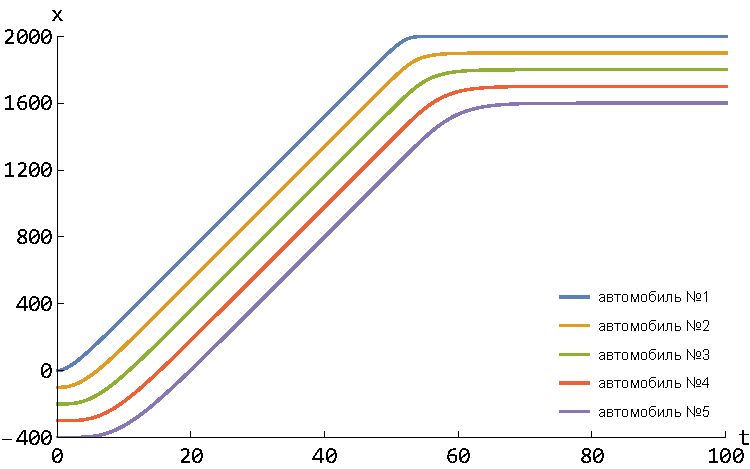
\includegraphics[width=1\linewidth,height=0.2\textheight]
			{Images/new_model_distanse.pdf}
		\end{minipage}
		\caption{Графики изменения скорости (слева) и расстояния (справа) для новой модели с параметрами: $a=0.5$, $q=0.6$, $v_{max}=40$, $v_{min}=0$, $\lambda=100$, $l=90$, $L=2000$, $x_0=0$, $v_n=0$, $g=9.8$, $\mu=0.6$ }
		\label{new_model_picture}
	\end{center}
\end{figure}

На графиках видна динамика, которая согласуется с динамикой реального транспортного потока. Автомобили разгоняются до максимальной допустимой скорости, а затем останавливаются на безопасном расстоянии. 

Модель \eqref{my_model} согласуется с реальной наблюдаемой ситуацией только на небольшом расстоянии между транспортными средствами, так как на большом расстоянии автомобилю нет смысла подстраивать свою скорость под скорость впереди идущей машины. Введём понятие \textbf{``расстояние влияния''}, под которым будем понимать такое расстояние, начиная с которого впереди идущий автомобиль оказывает влияние на позади идущий. В качестве ``расстояние влияния'' можно взять двойной тормозной путь $2S$. Таким образом, если расстояние между автомобилями большем, чем  $2S$, то преследующий автомобиль старается максимизировать свою скорость, если меньше, чем  $2S$, то преследующий автомобиль подстраивает свою скорость относительно впереди идущего. Математически это можно записать в виде релейной функции:

\begin{equation*}
F(\Delta x_{n}(t,\tau))=
\begin{cases}
\begin{split}
&v_{max},\quad &\text{если }\Delta x_{n-1,n}(t,\tau) > 2\dfrac{\dot{x}_n^2(t)}{2\mu g} \\
&\dot{x}_{n-1}(t-\tau),\quad &\text{если }\Delta x_{n-1,n}(t,\tau) \leq 2\dfrac{\dot{x}_n^2(t)}{2\mu g}
\end{split}
\end{cases}.
\end{equation*}

В реальной жизни максимальная комфортная скорость может быть своя у каждого автомобиля $v_{n,max}$, поэтому в некоторых случаях может возникнуть ситуация, когда впереди идущее транспортное средство движется со скоростью больше, чем максимальная комфортная скорость позади идущего. Для решения такой проблемы к первому слагаемому можно применить функцию Хевисайда \cite{Heaviside_function}, вида:
\begin{equation*}
\theta(\dot{x}_n(t))=
\begin{cases}
\begin{split}
&v_{n,max},\quad &\text{если }\dot{x}_n(t)>v_{n,max} \\
&\dot{x}_n(t),\quad &\text{если }\dot{x}_n(t)>v_{n,max}
\end{split}
\end{cases}.
\end{equation*}

Полученная математическая модель транспортных потоков согласуется с динамикой реального транспортного потока, и описывает все автомобили, включая первый и может быть применена для описания реальной дорожной ситуации.

\section{Практическое применение новой математической модели} 

\subsection{Подбор параметров} 

Прежде чем применять новую математическую модель \eqref{new_model} для моделирования реального транспортного потока, необходимо ввести систему единиц измерения для параметров, использующихся в модели.

Размерности для времени, расстояния и скорости возьмём из международной системы единиц (СИ). Таким образом, время будем измерять в секундах (с), расстояние в метрах (м), а скорость в метрах в секунду (м/с).

В системе \eqref{my_model} присутствуют константные параметры, значение которых можно определить заранее на основе физических законов, действующего законодательства Российской Федерации и логических соображений.

Параметр $v_{max}$ описывает максимальную желаемую скорость. В качестве максимального значения для параметра $v_{max}$ рассмотрим максимальную разрешённую скорость движения в населённом пункте \cite{PDD}, которая, согласно правилам дорожного движения, составляет 60 км/ч, что в системе СИ равняется примерно 16.7 м/с. Таким образом, $v_{max} \in [0,16.7]$. Параметр $v_{min}$ описывает минимальную желаемую скорость и ограничен лишь параметром $v_{max}$, таким образом, $v_{min} \in [0,v_{max}]$. В дорожных ситуациях данные параметры будут иметь конкретные значения.

Параметр $\lambda$, который описывает начальное расстояние между двумя соседними автомобилями, будем считать равным 3м \cite{PDD}, а параметр $l$ возьмём равным 2 м.

Параметр $\tau$, который описывает время реакции водителя, будем считать равным 1 с \cite{PDD}.

Коэффициент трения $\mu$ возьмём равный коэффициенту трения шин автомобиля по сухому асфальту $\mu=0.6$ \cite{Physics}

Ускорение свободного падения $g$ на поверхности Земли равно приблизительно $9.8 \text{ м/с}^2$.

Параметры $a$ и $q$ являются вычисляемыми и не имеют размерности. Подберём эти параметры эмпирически, исходя из наблюдаемых закономерностей. В среднем автомобиль разгоняется до скорости 60 км/ч за 7 с, такое ускорение достигается при $a\approx1$. Автомобиль, сбрасывая скорость до полной остановки, должен проехать расстояние равное тормозному пути, это достигается при $q\approx1$. Таким образом, коэффициенты $a$ и $q$ можно сделать равными $1$ и убрать из системы, так как на динамику реального транспортного потока они оказывают минимальное влияние.

Начальные параметры, такие как расстояние до препятствия $L$, начальное положение первого автомобиля $\lambda_0$, начальные скорости автомобилей потока $v_n$ могут быть любыми, так как они зависят от конкретной дорожной ситуации и не влияют на динамику движения транспортного потока.

Объединим все полученные параметры и запишем их в виде таблицы \ref{real_parameters}:
\begin{table}[h!]
	\caption{Значения константных параметров для модели \eqref{new_model} }
	\label{real_parameters}
	\begin{center}
		\begin{tabularx}{\textwidth}{p{0.12\linewidth}p{0.52\linewidth}p{0.11\linewidth}p{0.15\linewidth}}			
			\hline
			\rule{0cm}{0,5cm}
			Символ & Описание & Значение & Единица СИ \\
			[3pt]\hline
			$v_{max}$ & максимальная желаемая скорость& $[0,16.7]$&м/с\\
			$v_{min}$ & минимальная желаемая скорость& $[0,v_{max}]$&м/с\\ 
			$\tau$ & время реакции водителя& 1&с\\
			$\lambda$ & начальное расстояние между автомобилями& 3&м\\
			$l$ & расстояние между автомобилями& 4&м\\
			$g$ & ускорение свободного падения& 9.8&$\text{м/с}^2$\\ 
			$\mu$ &  коэффициент трения& 0.6& безразмерная\\ 
			\hline
		\end{tabularx}
	\end{center}
\end{table}
\newline 

\subsection{Применение новой математической модели в некоторых дорожных ситуациях}

Применять новую математическую модель в реальной дорожной ситуации затруднительно и затратно, поэтому некоторые дорожные ситуации были смоделированы при помощи компьютерных технологий. Для это была написана программа\footnote{Исходный код программы находится на диске в приложение \ref{att2}.} на языке программирования $Python$ версии 3.8.2 \cite{Python}. Для пользовательского интерфейса использовалась библиотека $Tkinter$, с модулем $ttk$ для расширения возможностей виджетов. Для визуализации графических данных использовалась библиотека научной графики $Matplotlib$ \cite{Matplotlib}.

Разработанная программа представляет собой оконное приложение, предназначенное для визуализации движения транспортных средств. В левой части расположены элементы управления приложением, с помощью которых пользователь может выбрать режим работы программы, задать некоторые начальные данные и запустить работу приложения. Правая часть предназначена, непосредственно, для визуализации движения автомобилей по дороге и для отображения графиков изменения скорости и пройденного пути для каждого автомобиля. На рисунке \ref{window} изображён интерфейс приложения. 

\begin{figure}[h!]  
	\begin{center}
		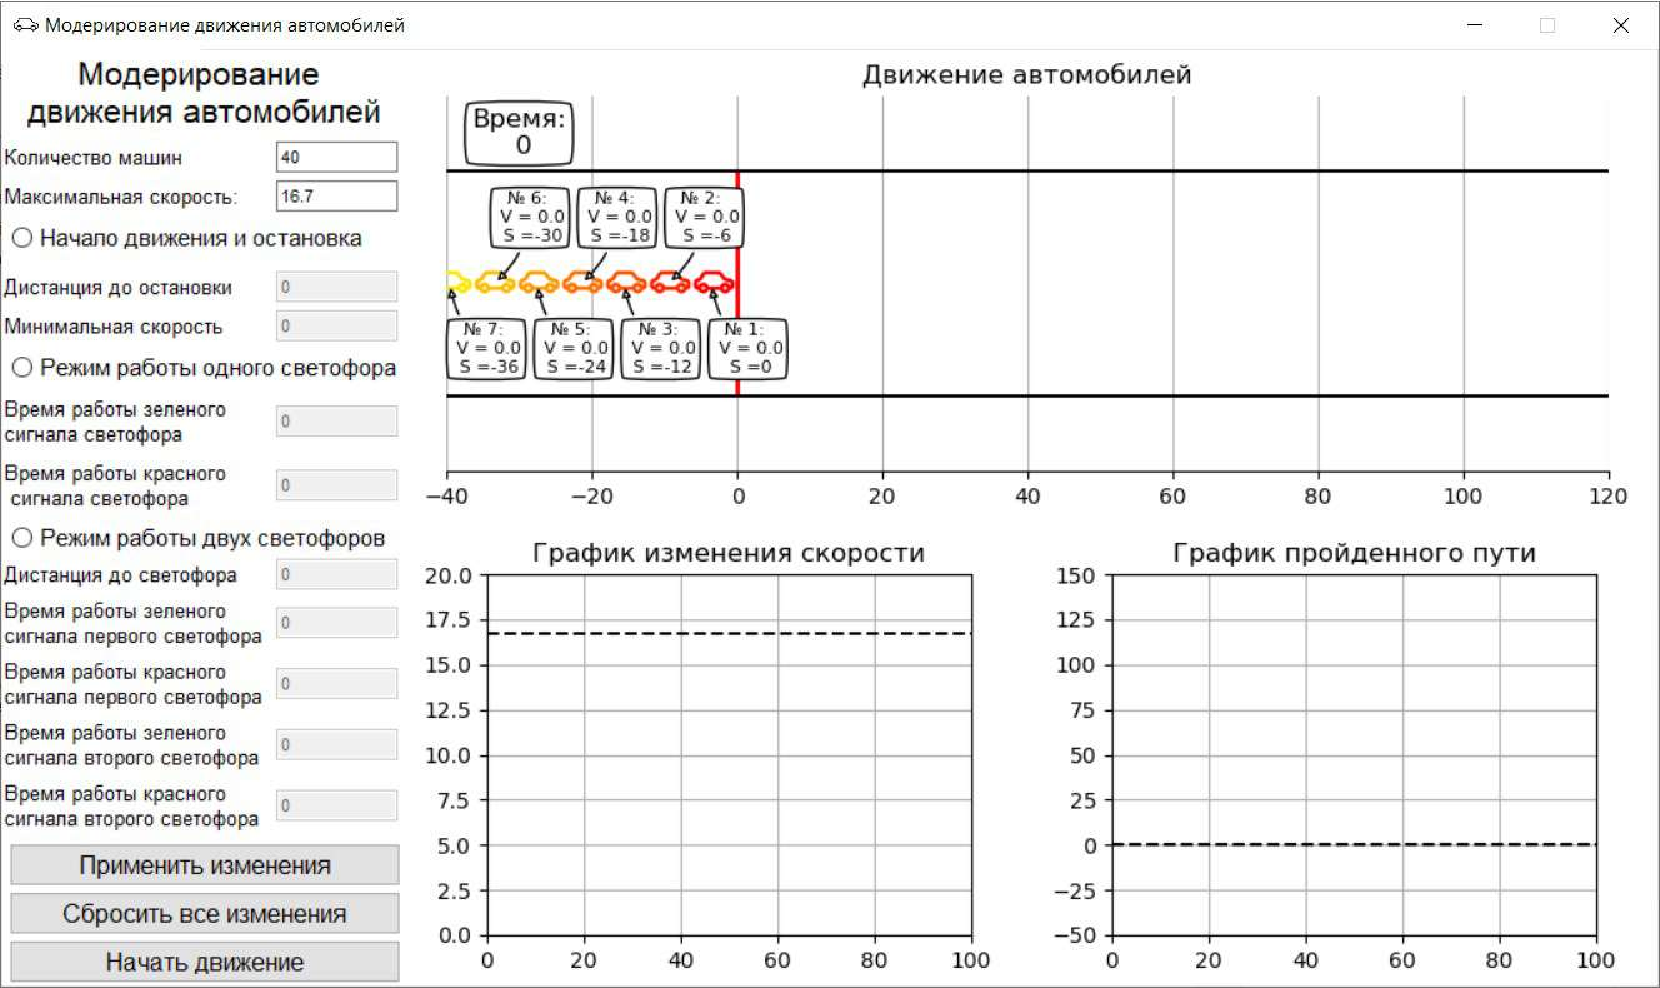
\includegraphics[keepaspectratio,width=160mm,height=70mm]
		{Images/screens/empty_window.pdf}
	\end{center}
	\caption{Интерфейс приложения.}
	\label{window}
\end{figure}

Для наглядности каждый автомобиль имеет свой цвет, причём графики изменения скорости и пройденного пути выполнены тем же цветом, что и автомобиль, которому они соответствуют. Так же для удобства рядом с каждым автомобилем отображается информация о его текущей скорости и пройденном пути. Началом отсчёта пройденного пути считается начальное положение первого автомобиля, таким образом, автомобили, которые не доехали до начального положения первого автомобиля, имеют отрицательное значение пройденного пути.

Автомобили в приложении двигаются согласно математической модели \eqref{my_model} с параметрами из таблицы \ref{real_parameters}. Для решения системы дифференциальных уравнений с запаздыванием в программе используется метод Рунге-Кутты \cite{Runge_Kutta}, адаптированный для уравнений с запаздыванием.

В начальный момент времени все автомобили стоят на безопасном расстоянии друг от друга. В модели \eqref{my_model} транспортные средства считались материальными точками и их размеры не учитывались, но для большей реалистичности в программе были использованы схематичные изображения автомобилей, которые, как и реальные транспортные средства, имеют размер. В данном случае габариты автомобиля равняются размеру его изображения. Эта величина прибавлена к константам $\lambda$ и $l$ и не оказывает влияния на динамику движения.

Полученная программа имеет три режима работы, каждый из которых позволяет смоделировать поведение автомобилей в конкретной дорожной ситуации. Для каждого режима есть свой набор начальных данных. ``Количество машин'' и ``максимальная скорость'' являются общими параметрами и указываются для каждого режима.

\noindent Таким образом, пользователь может смоделировать:

\begin{itemize} 
	\item \textit{начало движения и остановку автомобилей},
	\item \textit{режим работы одного светофора},
	\item \textit{режим работы двух светофоров}.
\end{itemize}

\noindent Рассмотрим каждый режим работы программы в отдельности.

\subsubsection{Начало движения и остановка}

Первый режим работы программы - это моделирование двух простых и информативных дорожных ситуаций, а именно, начало движения автомобиля и его торможение или остановка. Данные дорожные ситуации использовались для демонстрации применения всех моделей, рассмотренных в данной работе.

В этом режиме работы программы пользователь задаёт дистанцию, по достижению которой, автомобили должны сбросить скорость и значение минимальной скорости, до которой автомобили сбросят свою текущую скорость. В случае указания нулевого значения минимальной скорости машины остановятся.

На рисунках \ref{first_mode_1}, \ref{first_mode_2}, \ref{first_mode_3} и \ref{first_mode_4} изображены этапы работы программы в первом режиме.

\begin{figure}[h!]
	\begin{center}
		\begin{minipage}[h]{0.48\linewidth}
			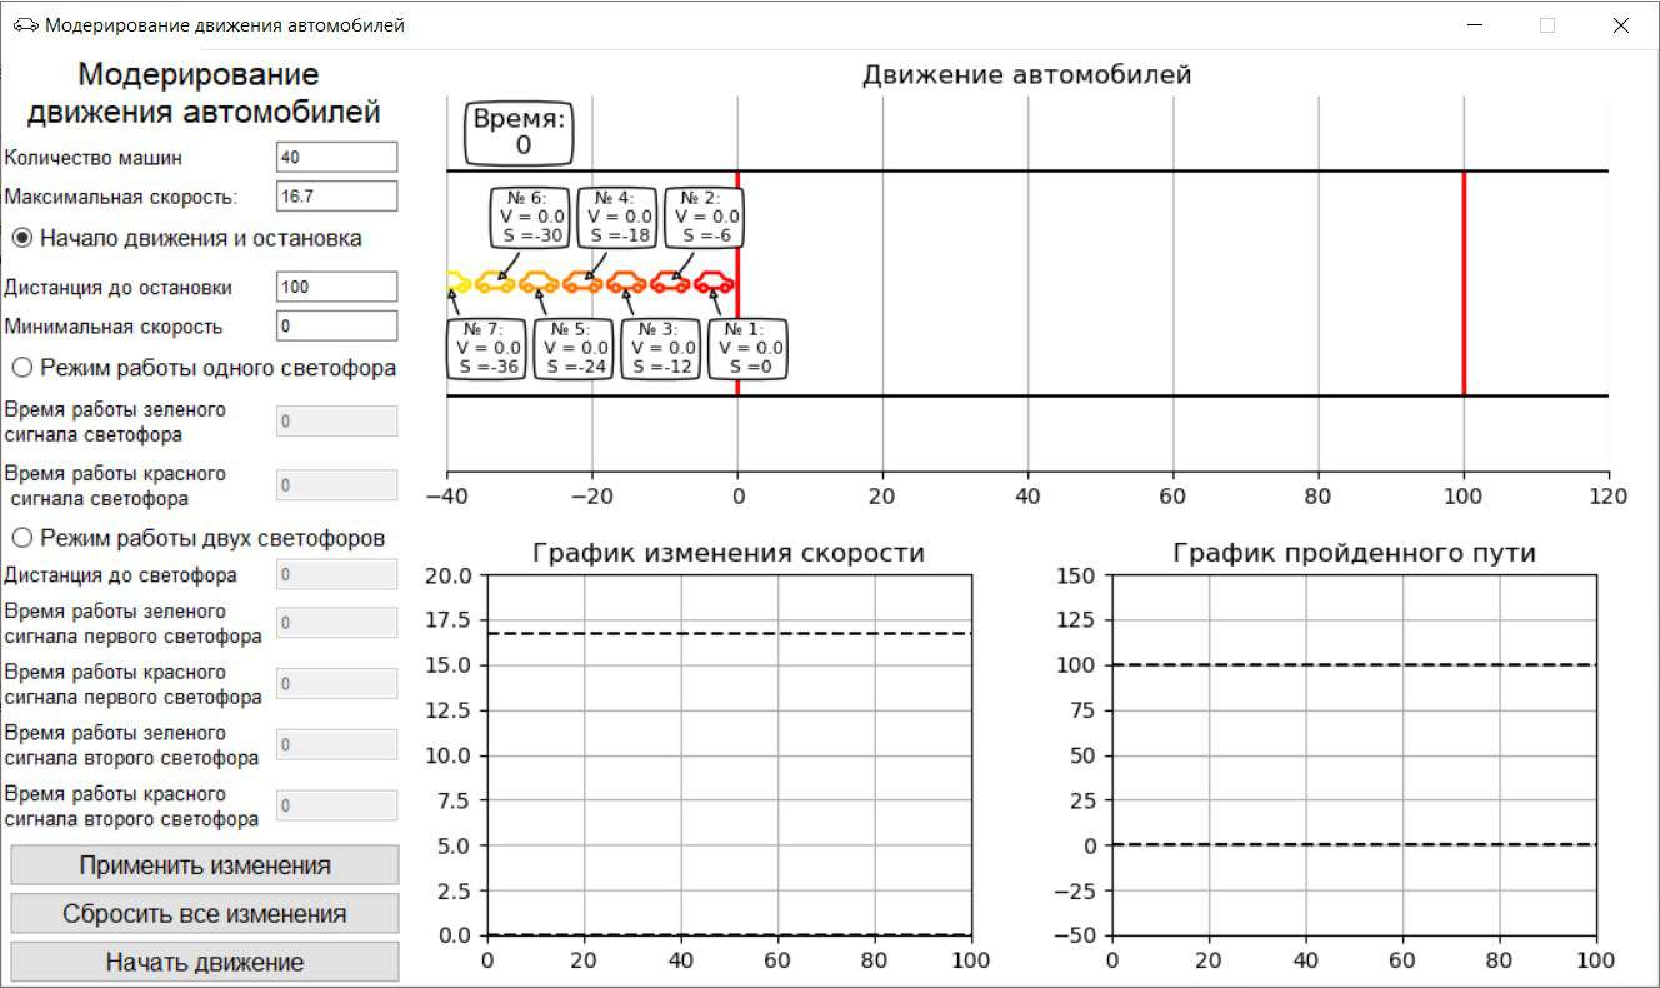
\includegraphics[width=1\linewidth]
			{Images/screens/first_mode_1}
			\caption{Положение автомобилей в нулевой момент времени.} 
			\label{first_mode_1}
		\end{minipage}
		\hfill 
		\begin{minipage}[h]{0.48\linewidth}
			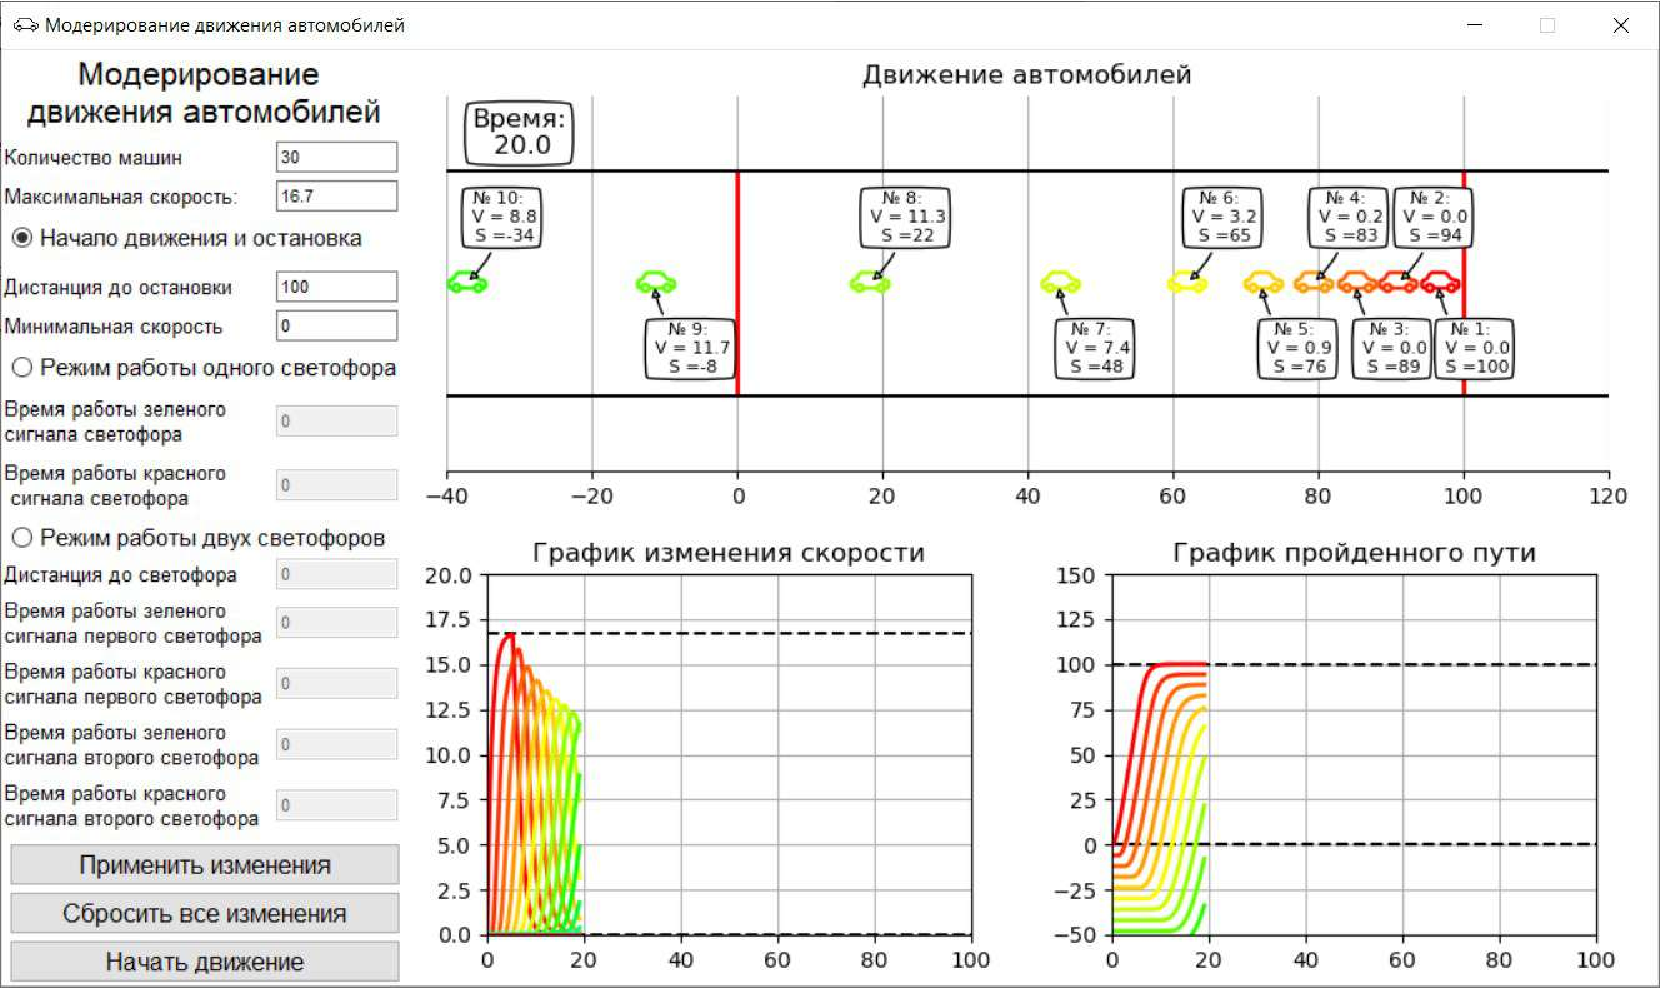
\includegraphics[width=1\linewidth]
			{Images/screens/first_mode_2}
			\caption{Положение автомобилей через 20 секунд после начала движения.}
			\label{first_mode_2}
		\end{minipage}
		\hfill 
		\begin{minipage}[h]{0.48\linewidth}
			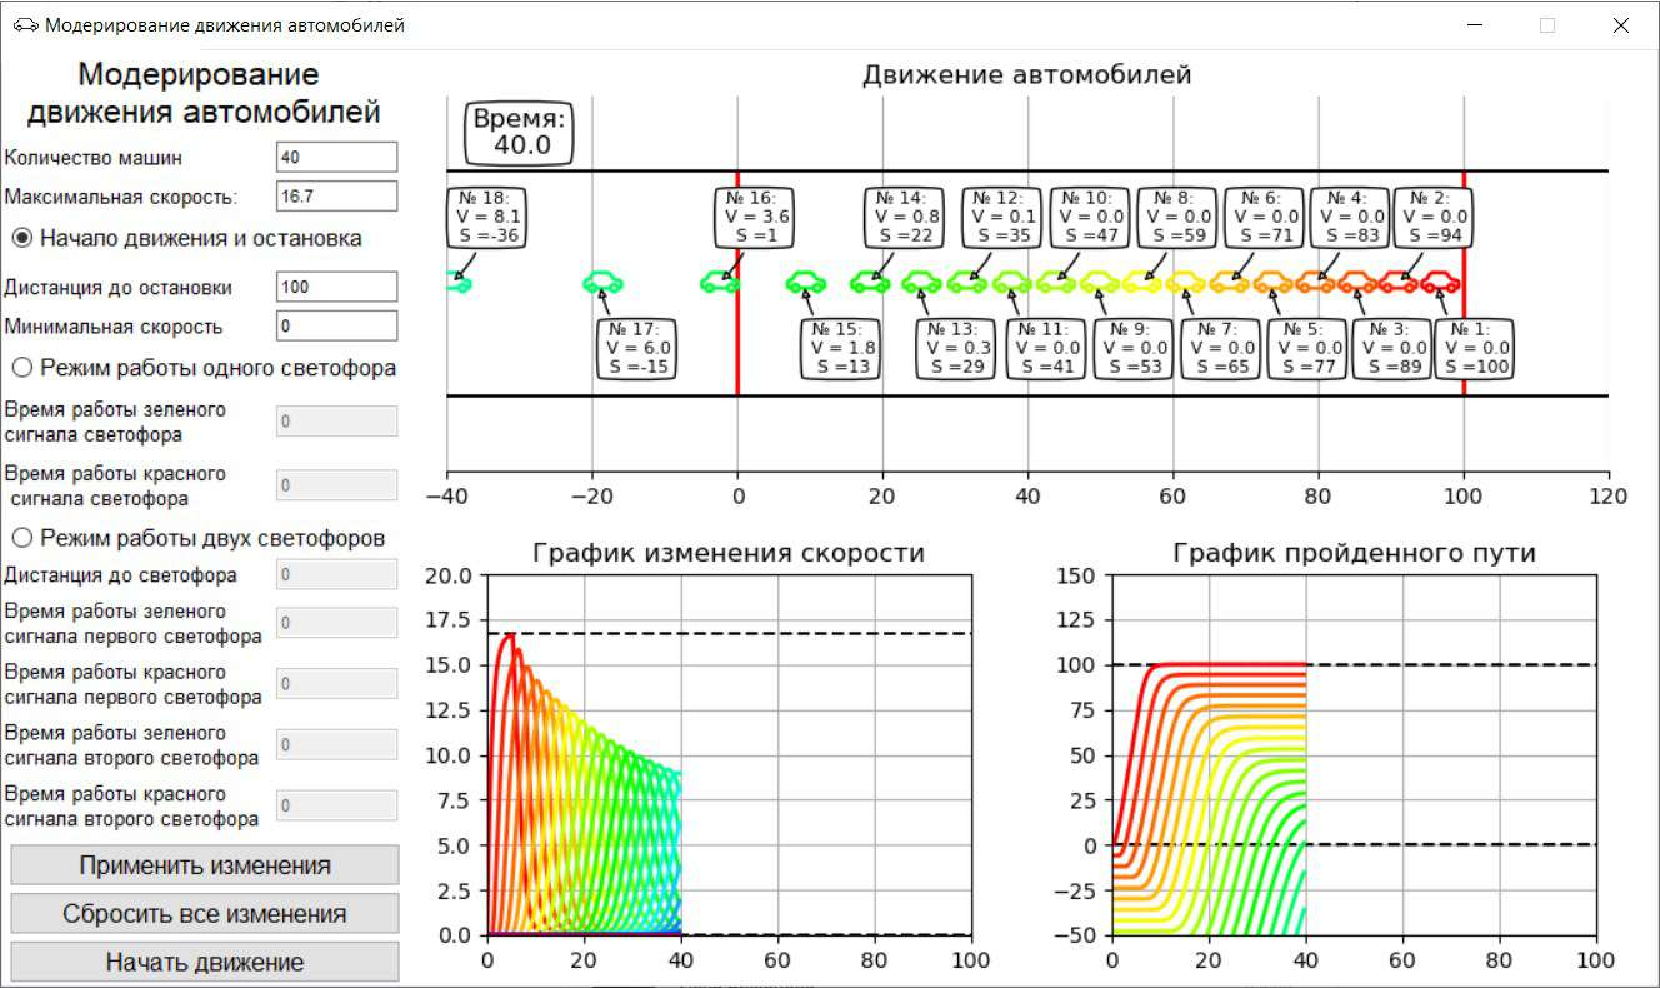
\includegraphics[width=1\linewidth]
			{Images/screens/first_mode_3}
			\caption{Положение автомобилей через 40 секунд после начала движения.}
			\label{first_mode_3}
		\end{minipage}
			\hfill 
		\begin{minipage}[h]{0.48\linewidth}
			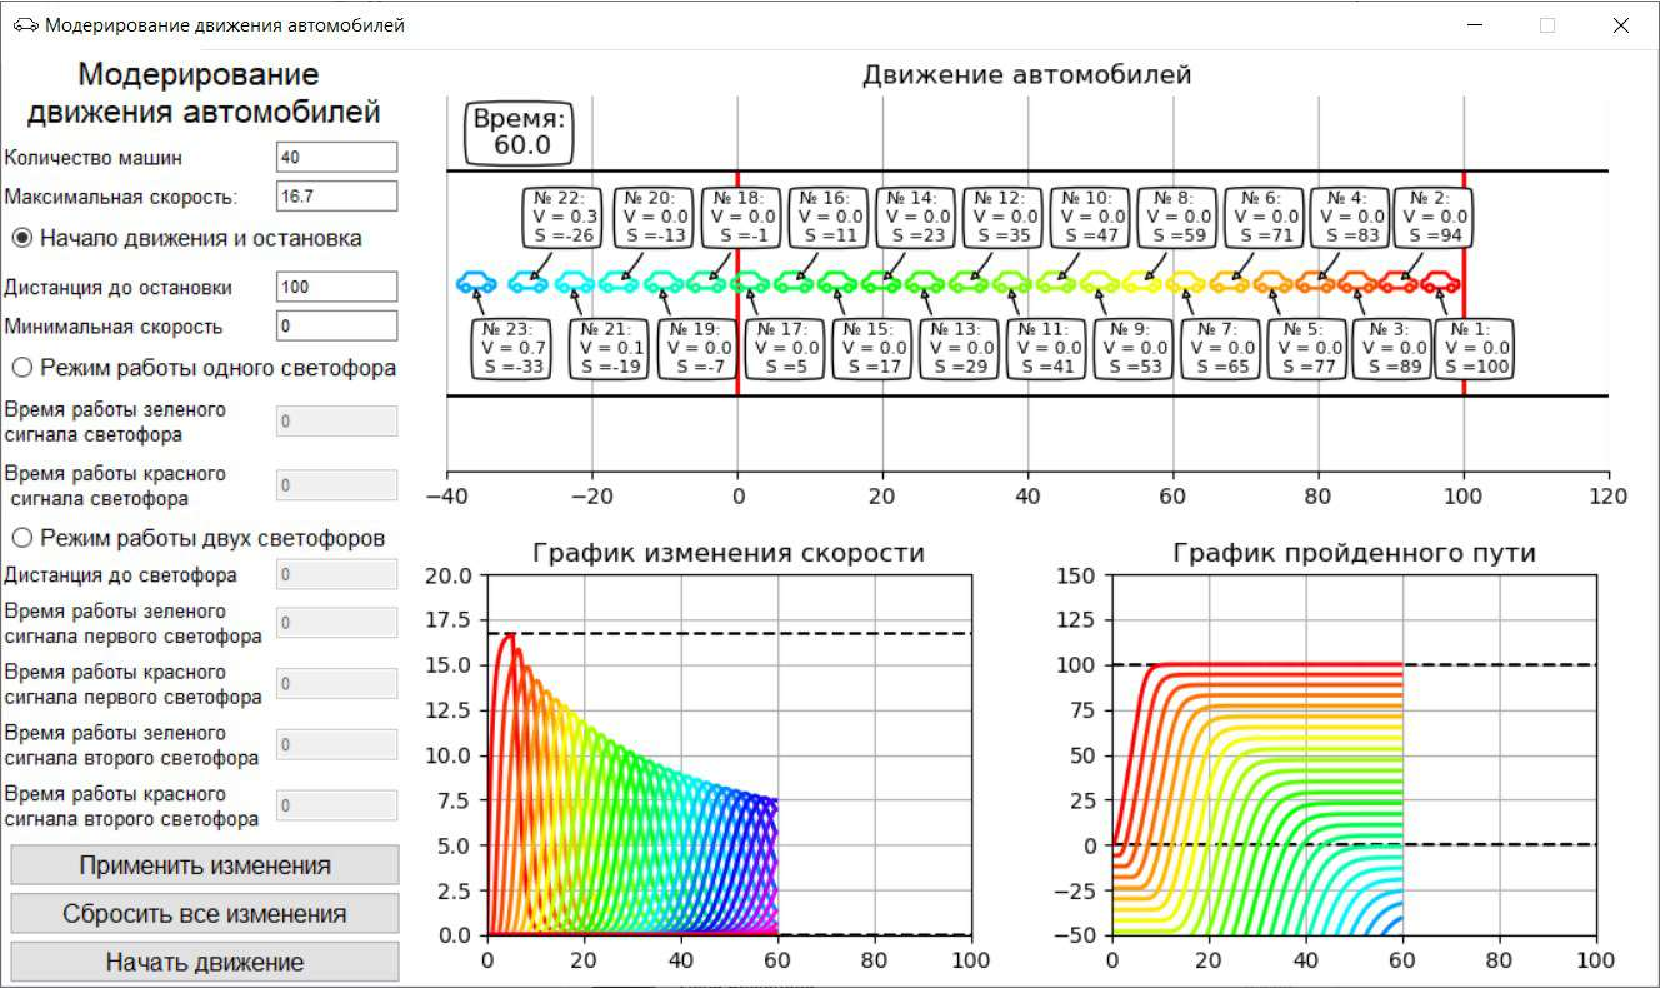
\includegraphics[width=1\linewidth]
			{Images/screens/first_mode_4}
			\caption{Положение автомобилей через 60 секунд после начала движения.}
			\label{first_mode_4}
		\end{minipage}
	\end{center}
\end{figure}

Из рисунков видно, что работа программы в данном режиме полностью согласуется с динамикой реального транспортного потока.

Данный режим работы программы подойдёт для моделирования участков дорог, где присутствует изменение скоростного режима.

\subsubsection{Режим работы одного светофора}

Второй режим работы программы - это моделирование режима работы одного светофора. Работа светофора состоит из циклов, которые в свою очередь состоят из двух фаз. Первая фаза определяется временным интервалом работы зелёного сигнала светофора, а вторая - красного. Именно эти параметры пользователь задаёт в данном режиме работы программы. Таким образом, пользователь указывает временные интервалы работы зелёного и красного сигналов светофора. 

Во время работы зелёного сигнала светофора автомобили проезжают через светофор, во время работы красного сигнала автомобили останавливаются перед светофором на безопасном расстоянии и ждут включения зелёного сигнала. 

Основным критерием работы светофора будем считать количество автомобилей, которые проехали через светофор за один цикл его работы, а именно за время работы зелёного сигнала. Иногда может возникнуть ситуация, когда в момент смены сигнала светофора расстояние между автомобилем и светофором меньшем, чем длинна тормозного пути. В таком случае, чтобы не применять экстренное торможение, автомобилю разрешается проехать светофор на запрещающий сигнал. Такое поведение согласуется с правилами дорожного движения \cite{PDD}.

На рисунках \ref{second_mode_1}, \ref{second_mode_2}, \ref{second_mode_3}, \ref{second_mode_4}, \ref{second_mode_6} и \ref{second_mode_9} показано применение программы для моделирования работы одного светофора, с характеристиками, наблюдаемыми у реального светофора (приложение \ref{att}).

\begin{figure}[h!]
	\begin{center}
		\begin{minipage}[h]{0.48\linewidth}
			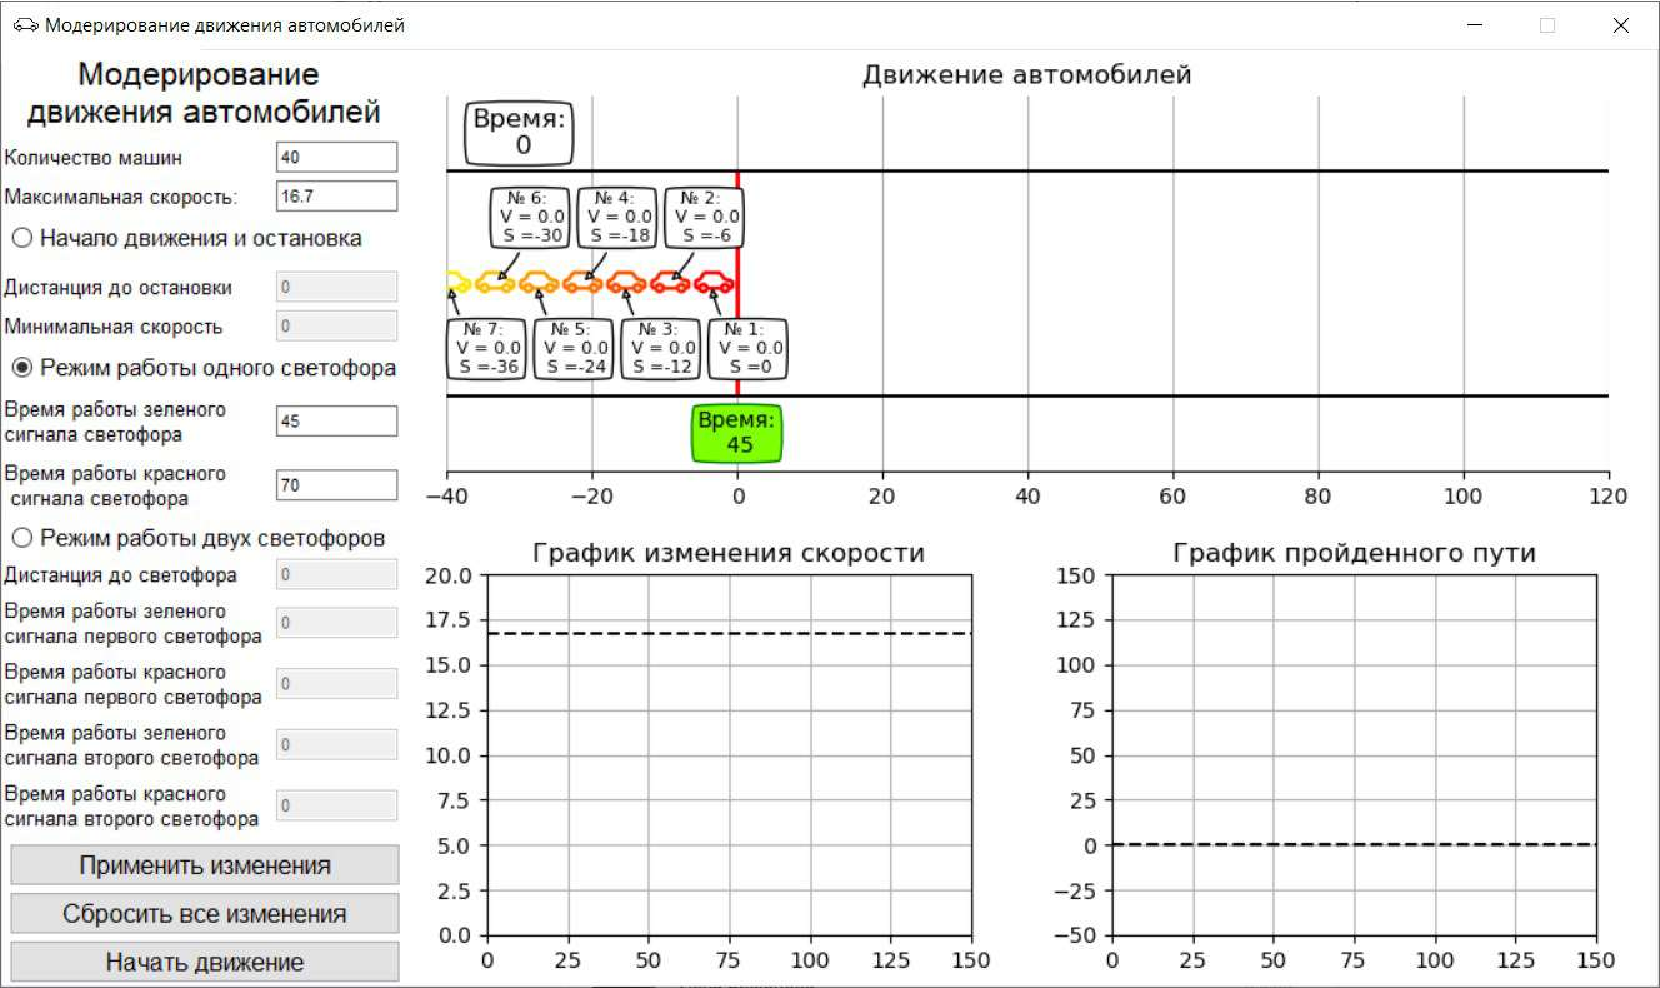
\includegraphics[width=1\linewidth]
			{Images/screens/second_mode_1}
			\caption{Положение автомобилей в нулевой момент времени.} 
			\label{second_mode_1}
		\end{minipage}
		\hfill 
		\begin{minipage}[h]{0.48\linewidth}
			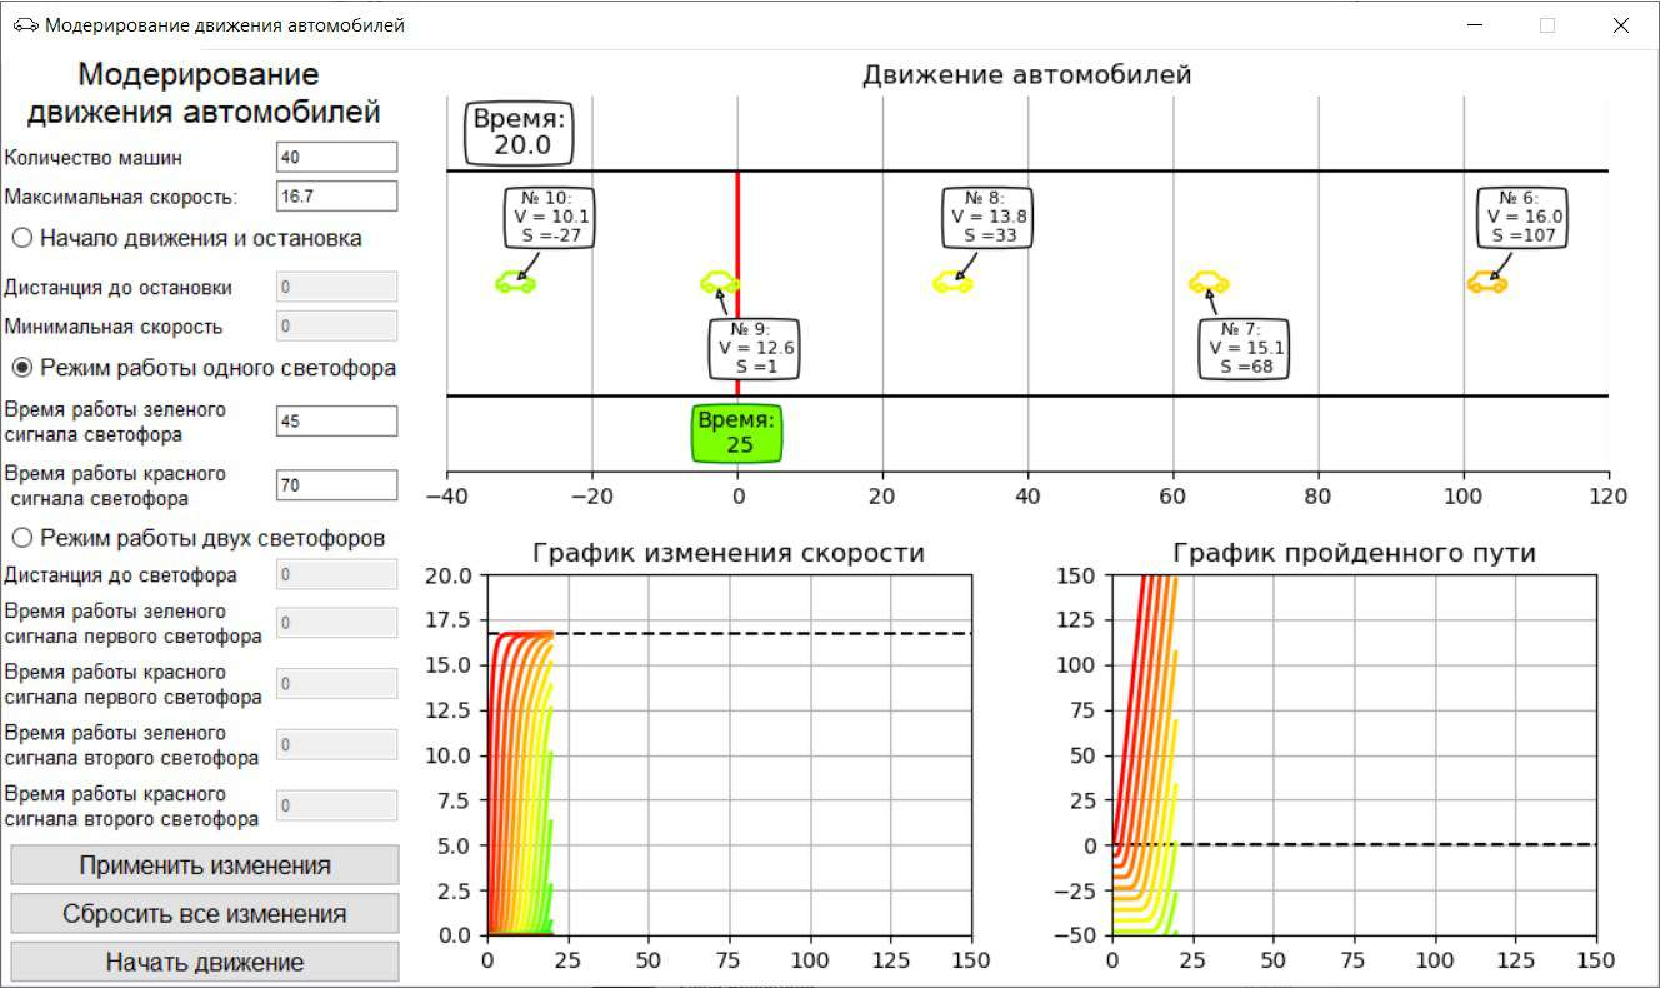
\includegraphics[width=1\linewidth]
			{Images/screens/second_mode_2}
			\caption{Положение автомобилей через 20 секунд после начала движения.}
			\label{second_mode_2}
		\end{minipage}
	\end{center}
\end{figure}
\begin{figure}[h!]
	\begin{center}
		\begin{minipage}[h]{0.48\linewidth}
			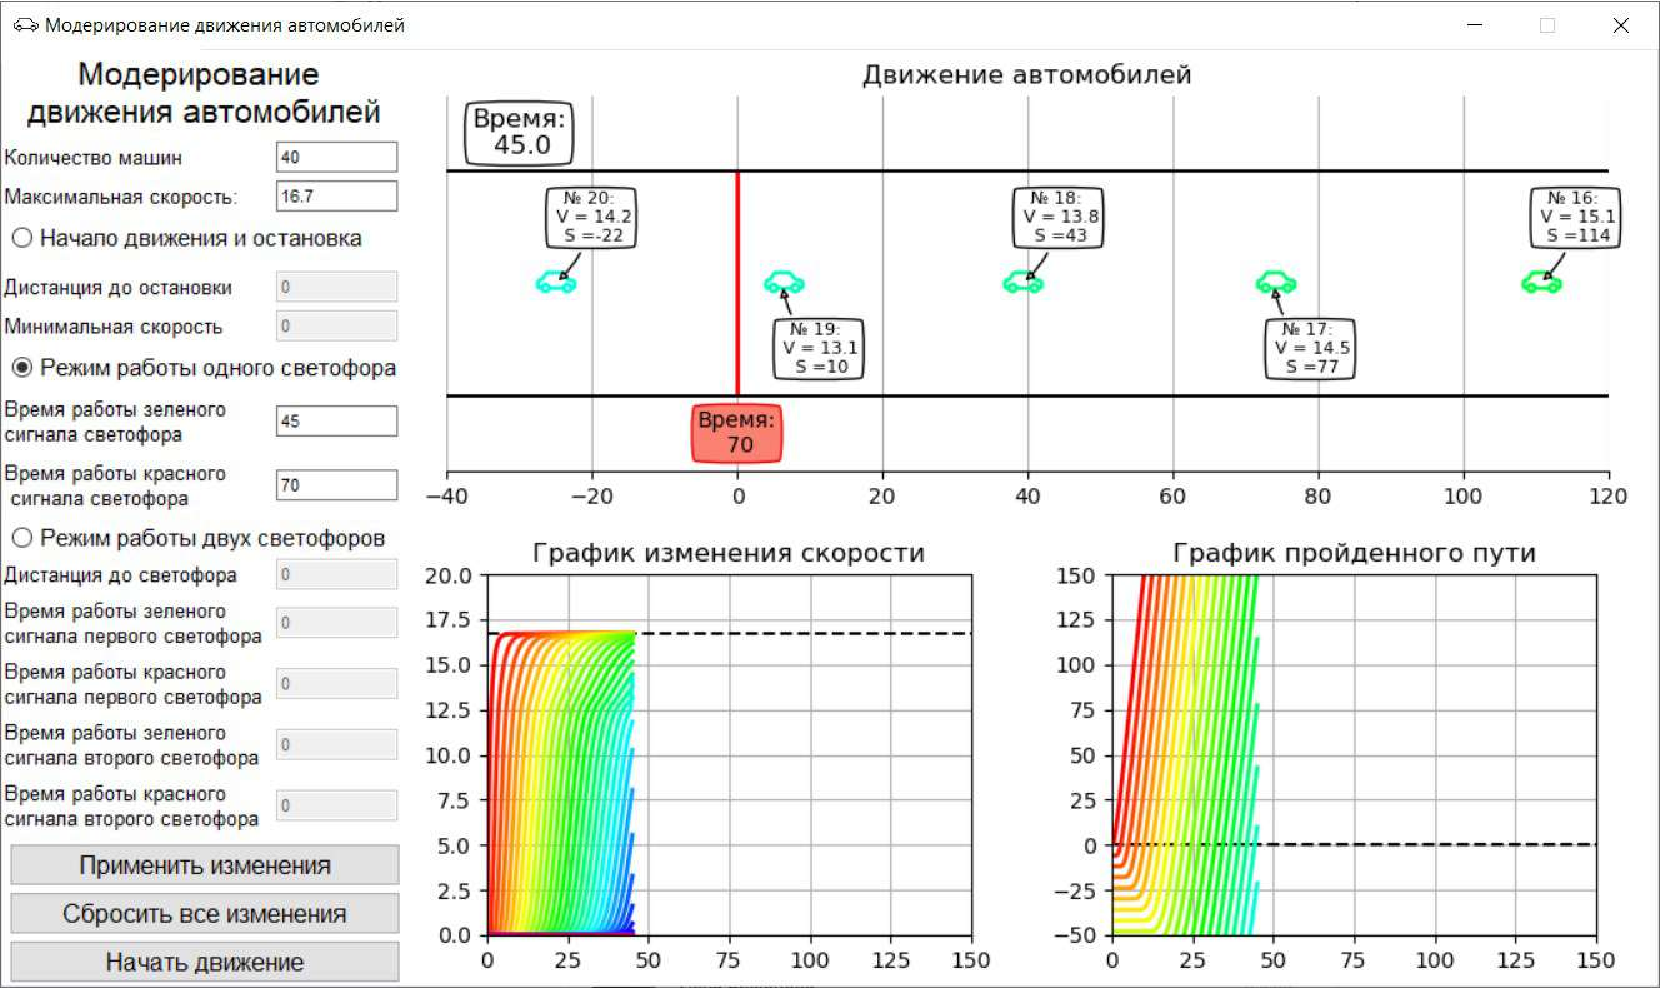
\includegraphics[width=1\linewidth]
			{Images/screens/second_mode_3}
			\caption{Положение автомобилей через 45 секунд после начала движения.}
			\label{second_mode_3}
		\end{minipage}
		\hfill 
		\begin{minipage}[h]{0.48\linewidth}
			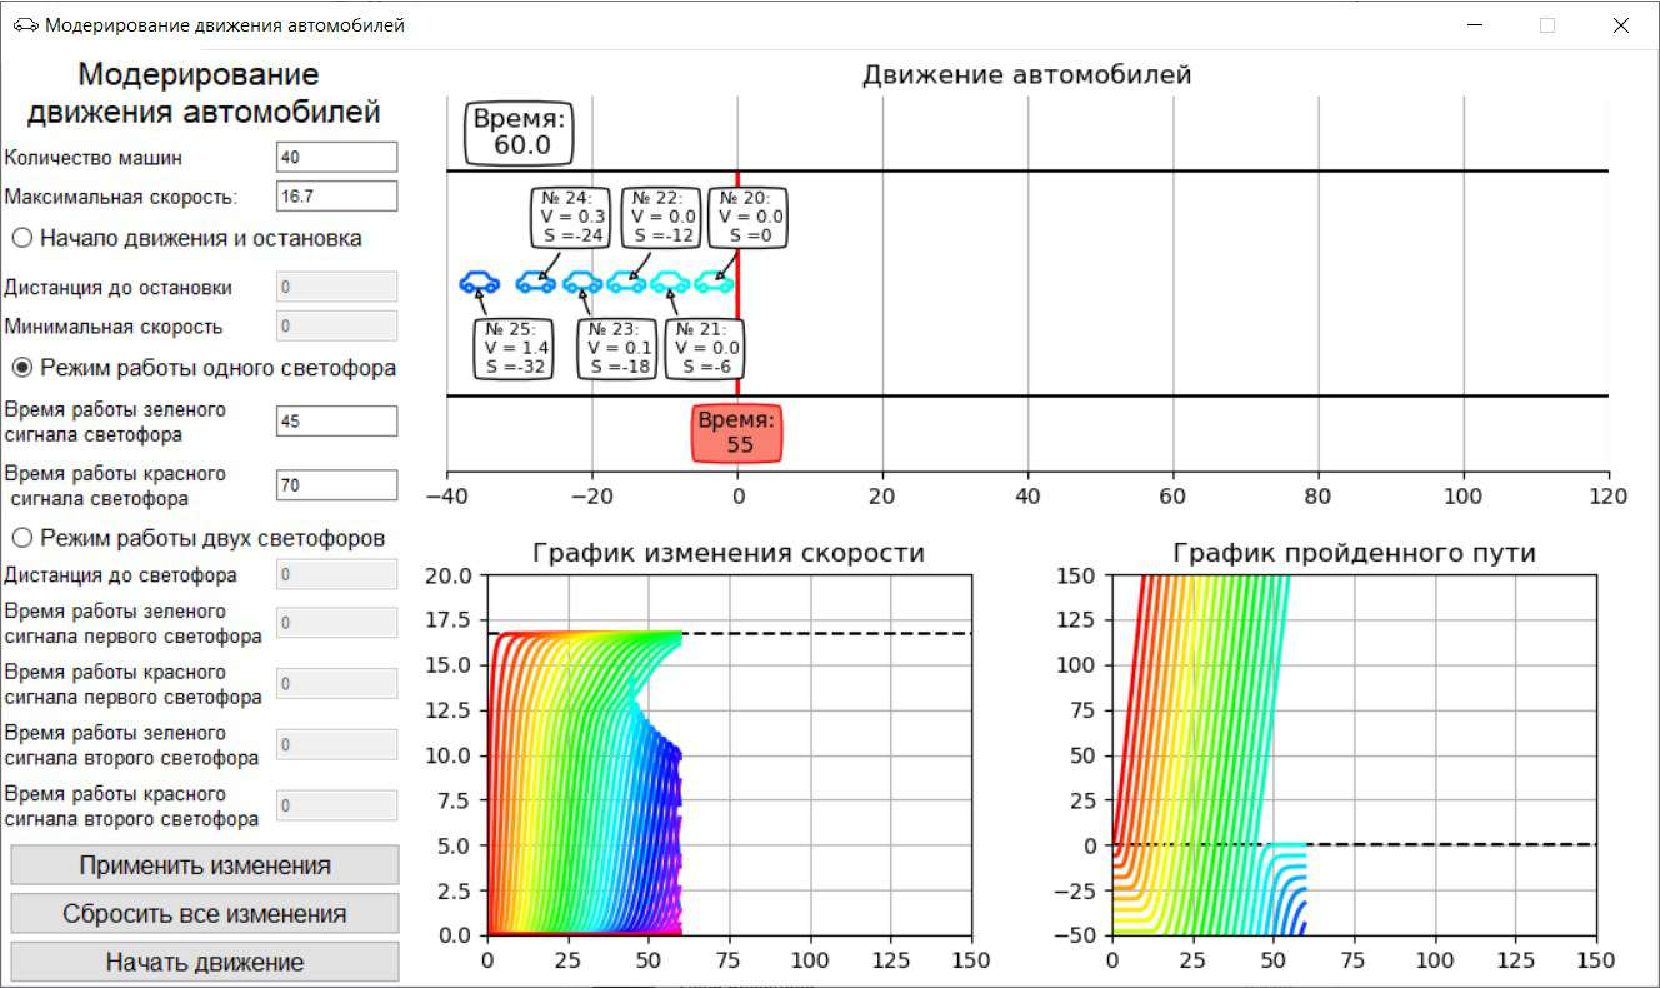
\includegraphics[width=1\linewidth]
			{Images/screens/second_mode_4}
			\caption{Положение автомобилей через 60 секунд после начала движения.}
			\label{second_mode_4}
		\end{minipage}
		\hfill
		\begin{minipage}[h]{0.48\linewidth}
			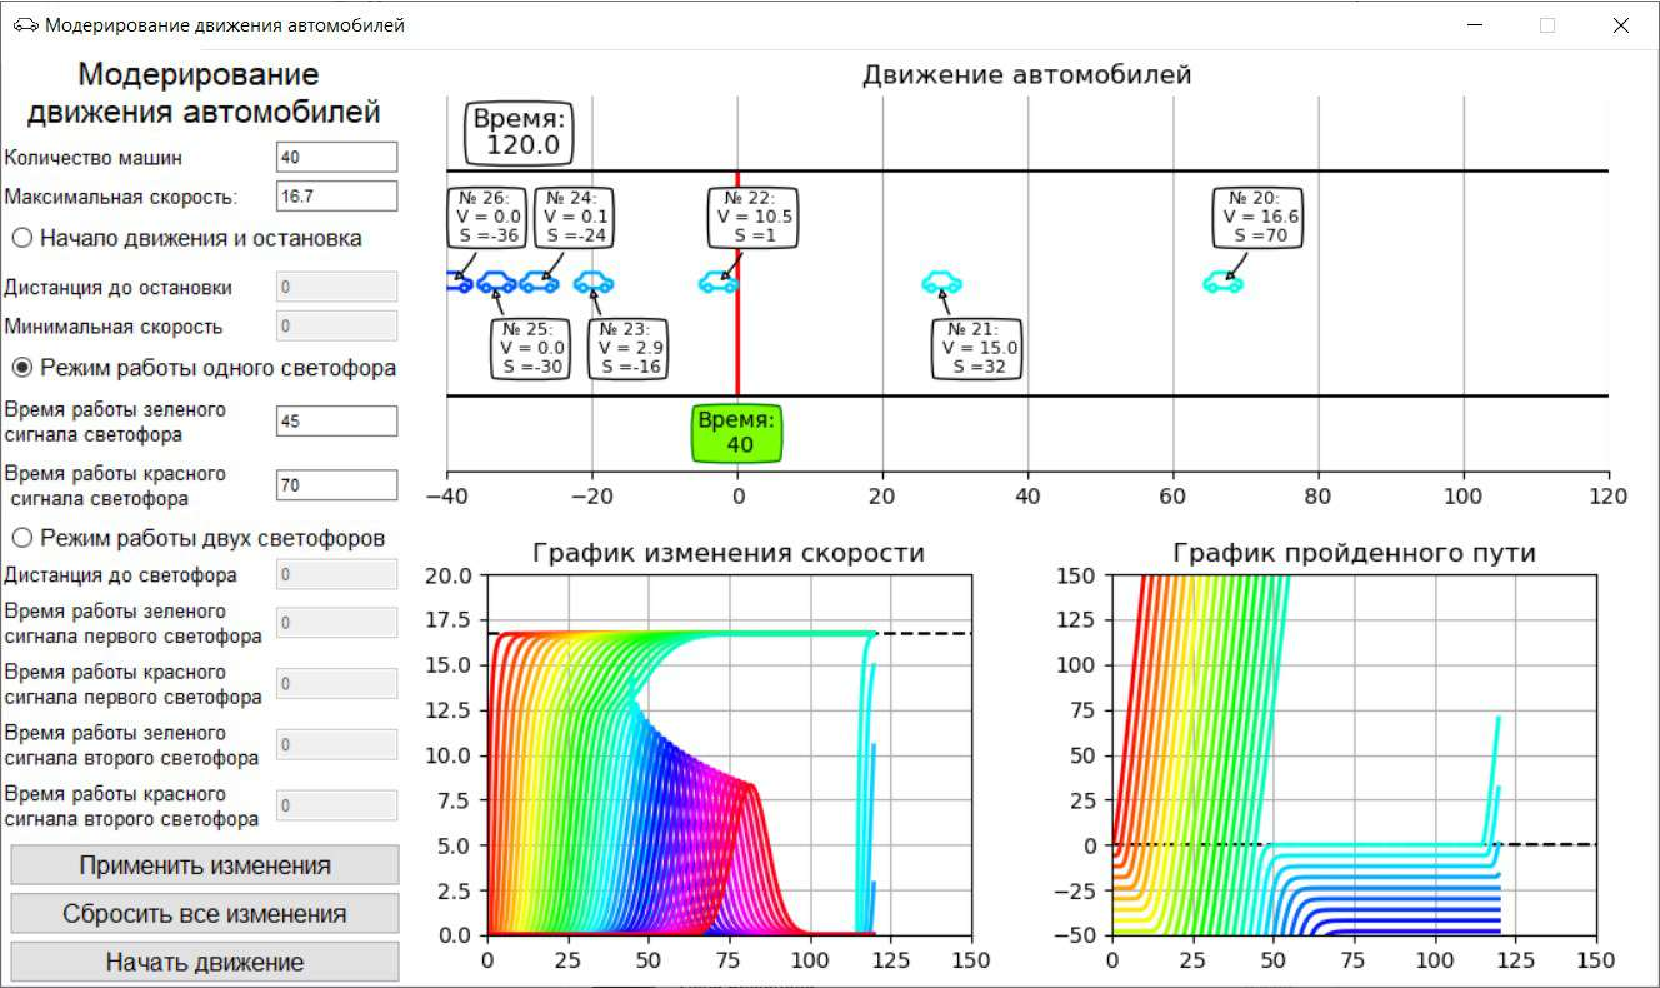
\includegraphics[width=1\linewidth]
			{Images/screens/second_mode_6}
			\caption{Положение автомобилей через 120 секунд после начала движения.}
			\label{second_mode_6}
		\end{minipage}
		\hfill
		\begin{minipage}[h]{0.48\linewidth}
			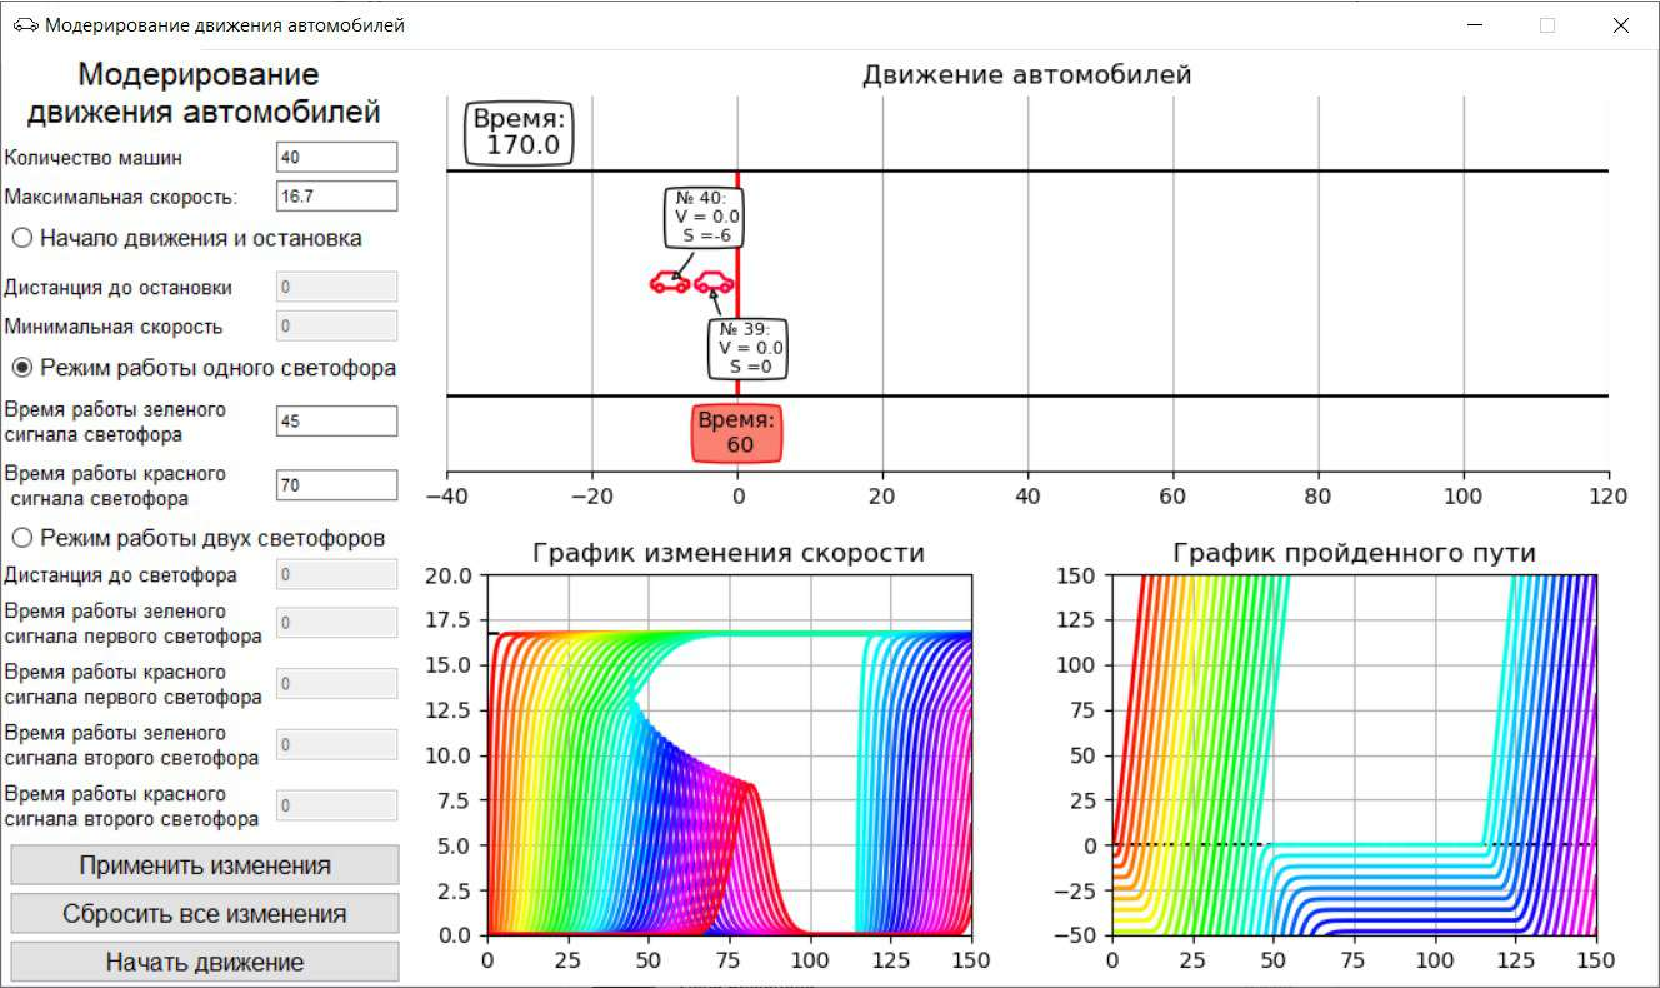
\includegraphics[width=1\linewidth]
			{Images/screens/second_mode_9}
			\caption{Положение автомобилей через 170 секунд после начала движения.} 
			\label{second_mode_9}
		\end{minipage}
	\end{center}
\end{figure}

На рисунках \ref{second_mode_1}, \ref{second_mode_2}, \ref{second_mode_3}, \ref{second_mode_4}, \ref{second_mode_6} и \ref{second_mode_9} показано моделирование нескольких циклов работы реального светофора. Как видно из рисунков количество автомобилей, которое проезжает через светофор в разработанном приложении равно среднему количеству автомобилей, которые проезжают через реальный светофор. Это подтверждает корректность и самой модели \eqref{my_model}, и правильность подбора параметров (таблица \ref{real_parameters}). 

Данный режим работы программы подойдёт для моделирования участков дорог со светофором. С его помощью можно отрегулировать режим работы светофора не опасаясь серьёзных последствий, таких как пробки, которые могли бы возникнуть при неудачной настройке реального светофора.  

\subsubsection{Режим работы двух светофоров}

Третий режим программы - это моделирование режима работы двух последовательно идущих светофоров. Светофоры в данном режиме не зависят друг от друга и работа каждого из них аналогична работе светофора, рассмотренной в предыдущем пункте. Соответственно, поведение автомобилей также остаётся аналогичным случаю одного светофора.

В данном режиме пользователь задаёт время работы зелёного и красного сигналов для каждого светофора и расстояние между ними. 

На рисунках \ref{third_mode_1}, \ref{third_mode_2}, \ref{third_mode_3}, \ref{third_mode_4}, \ref{third_mode_11} \ref{third_mode_12} \ref{third_mode_14} и \ref{third_mode_15} показано применение программы для моделирования работы двух последовательно идущих светофоров, с характеристиками, наблюдаемыми у двух реальных светофоров, идущих друг за другом (приложение \ref{att}).

\begin{figure}[H]
	\begin{center}
		\begin{minipage}[h]{0.48\linewidth}
			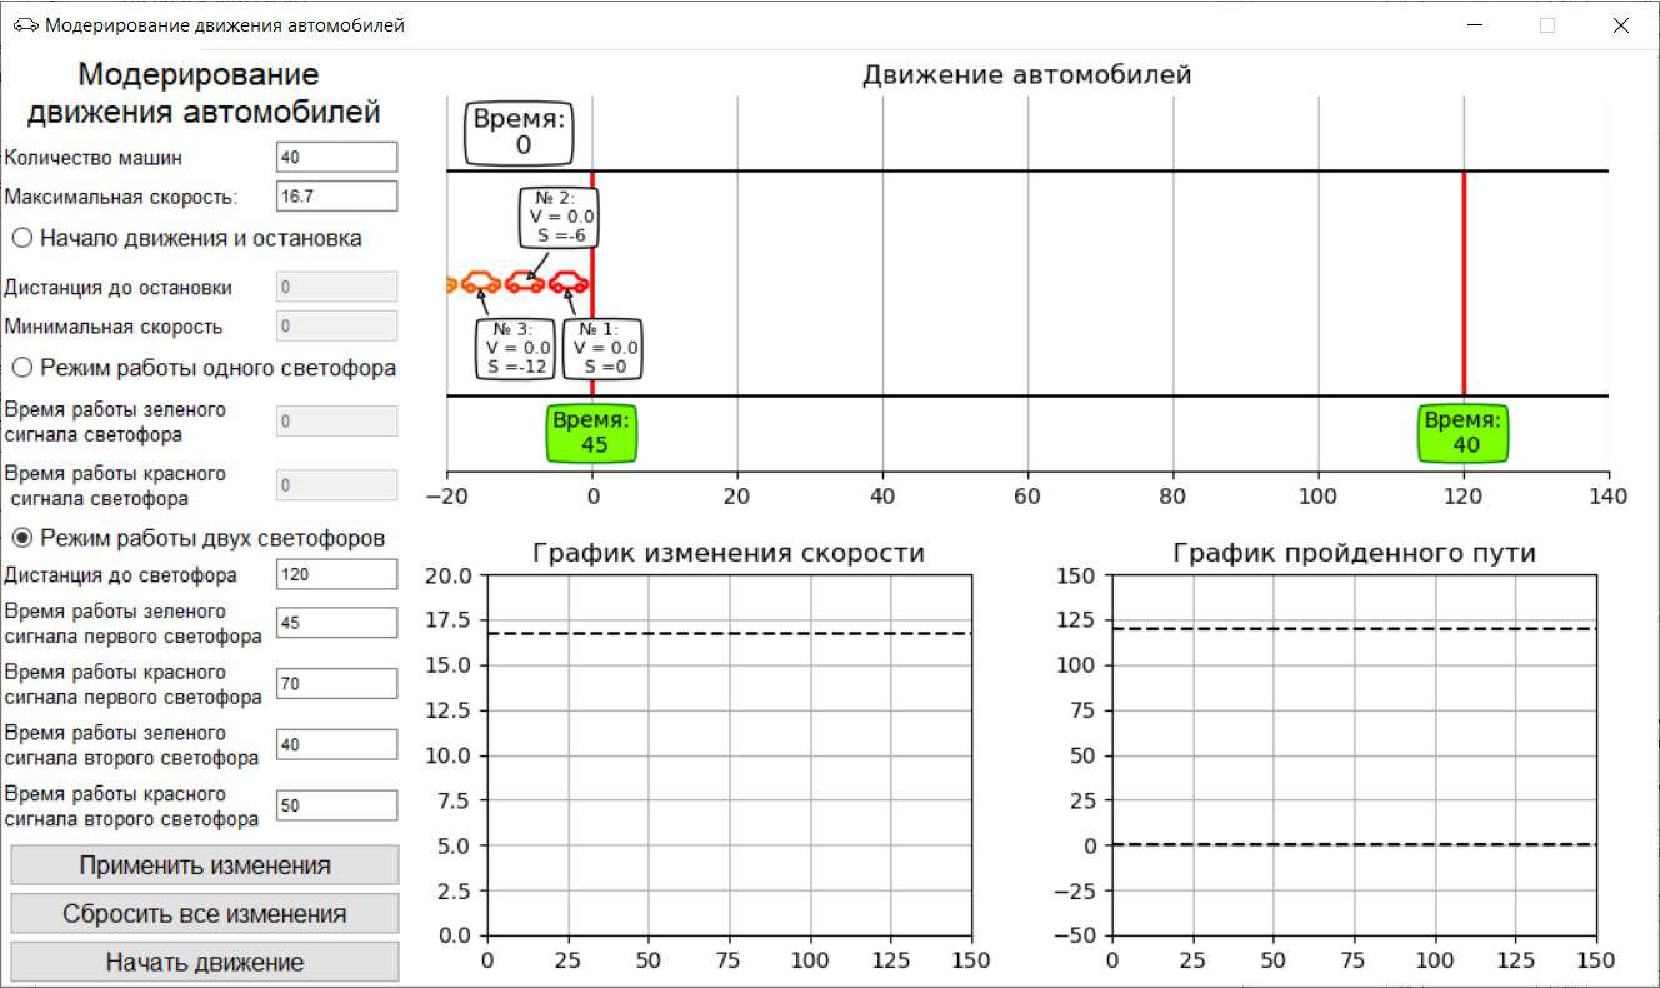
\includegraphics[width=1\linewidth]
			{Images/screens/third_mode_1}
			\caption{Положение автомобилей в нулевой момент времени.} 
			\label{third_mode_1}
		\end{minipage}
		\hfill 
		\begin{minipage}[h]{0.48\linewidth}
			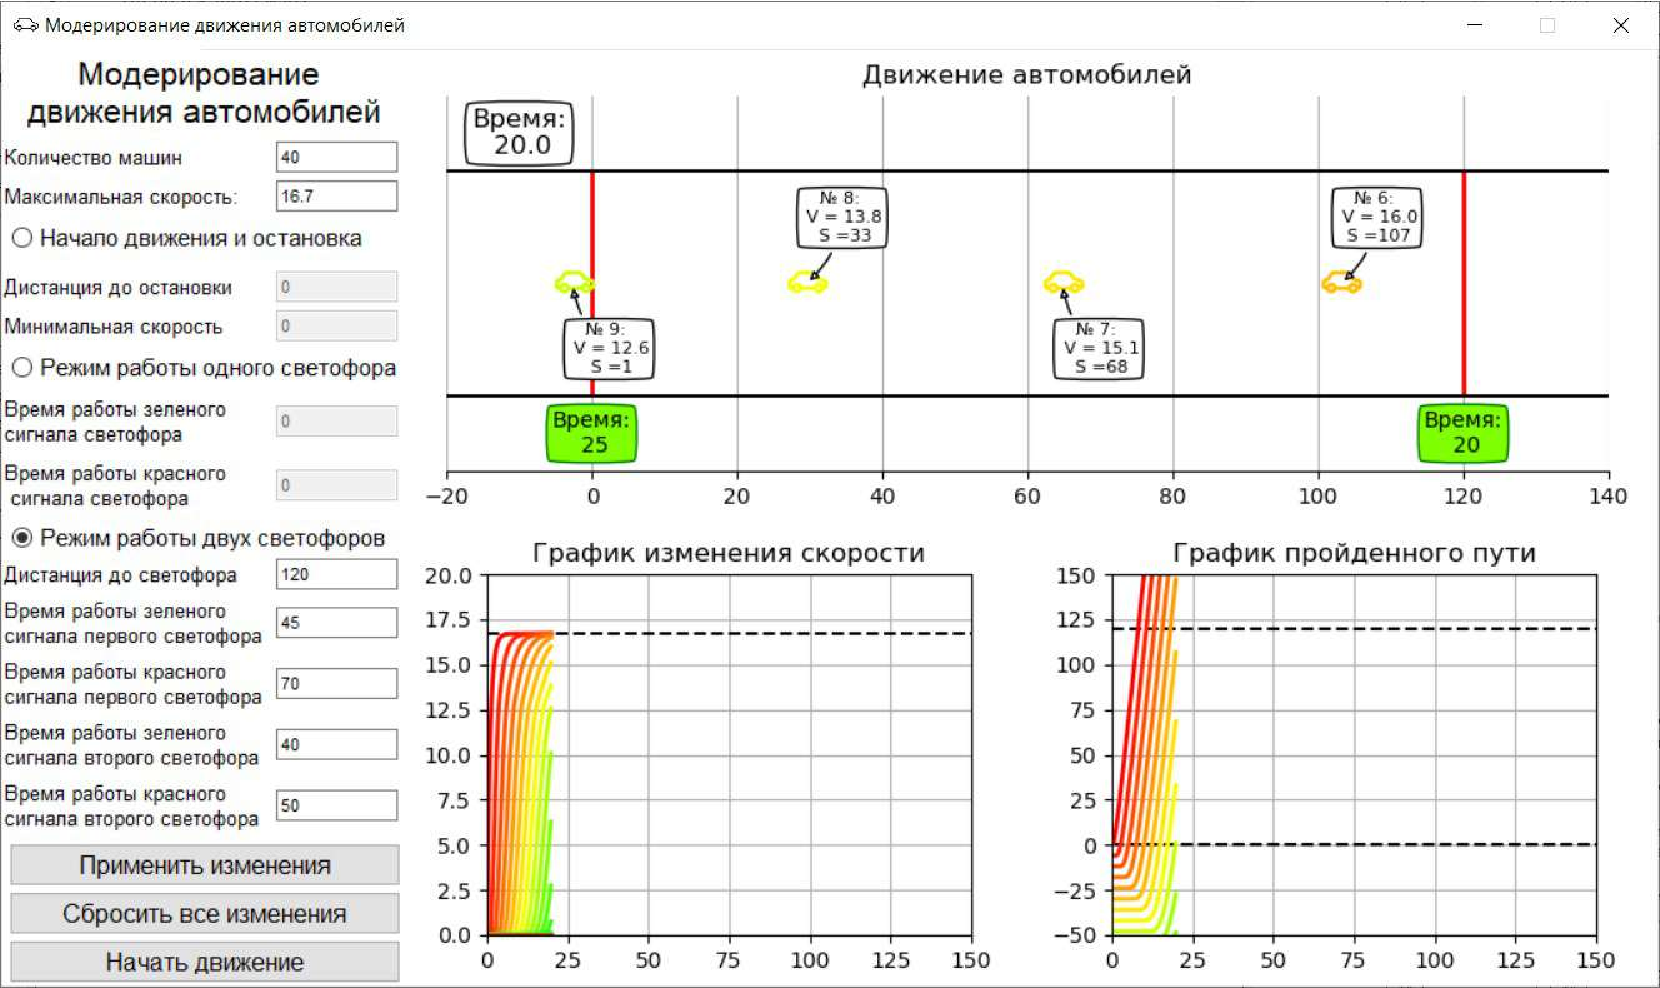
\includegraphics[width=1\linewidth]
			{Images/screens/third_mode_2}
			\caption{Положение автомобилей через 20 секунд после начала движения.}
			\label{third_mode_2}
		\end{minipage}
		\hfill 
		\begin{minipage}[h]{0.48\linewidth}
			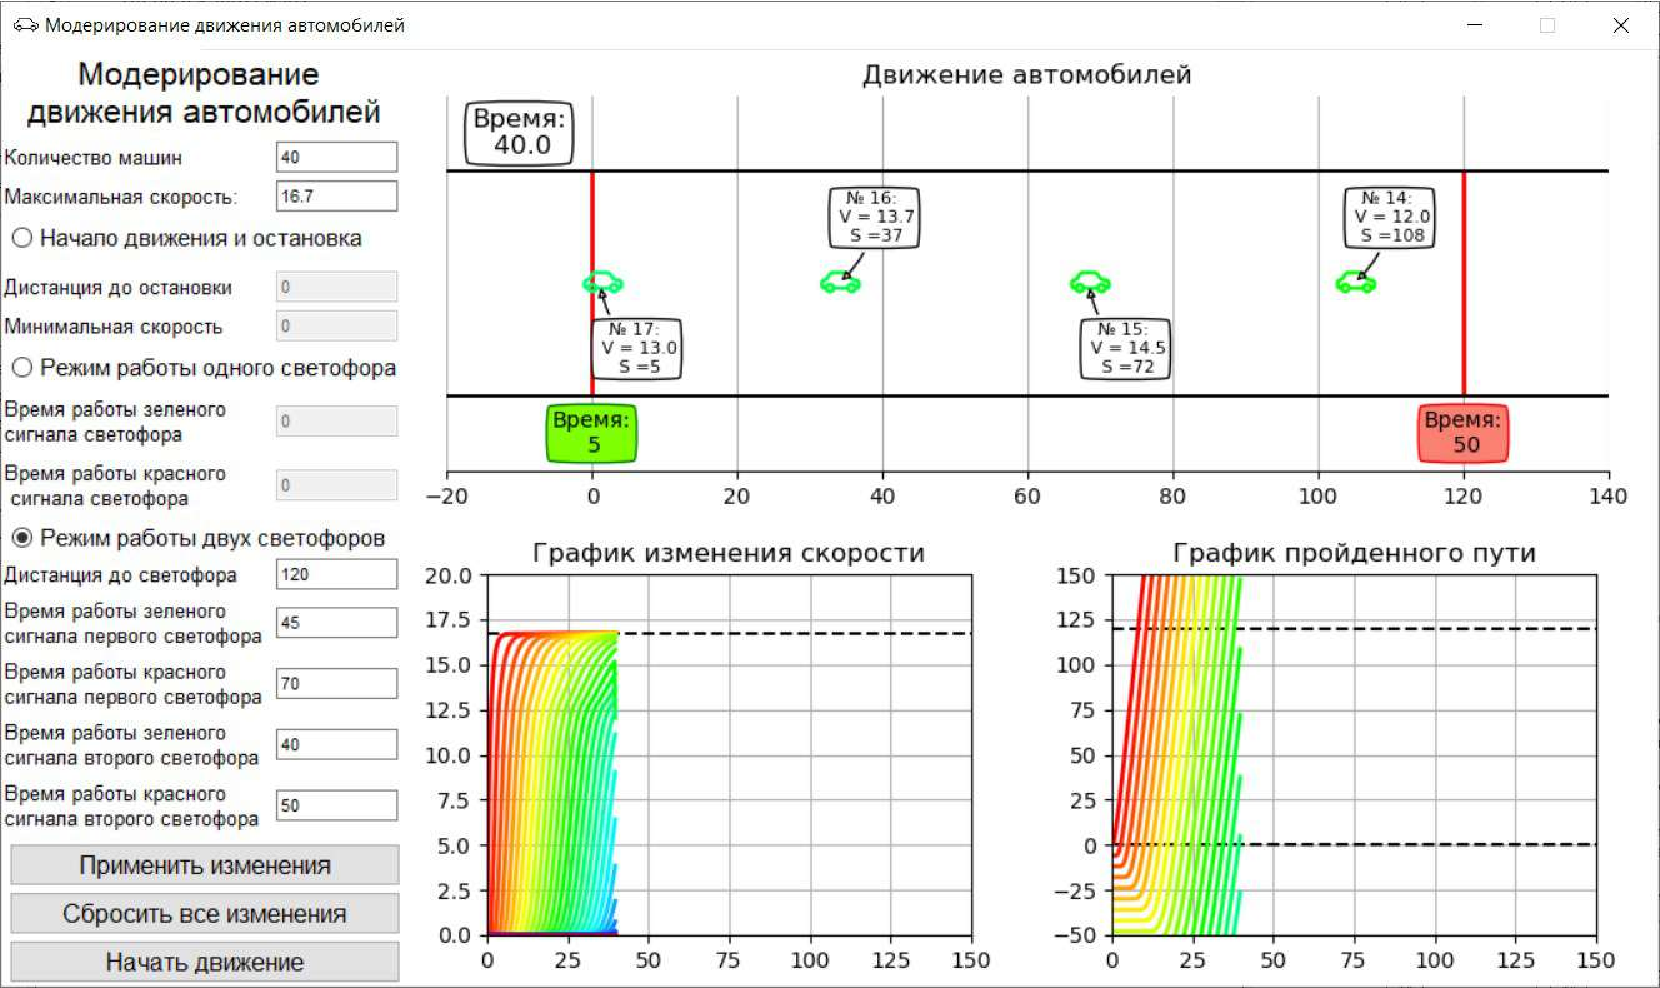
\includegraphics[width=1\linewidth]
			{Images/screens/third_mode_3}
			\caption{Положение автомобилей через 40 секунд после начала движения.}
			\label{third_mode_3}
		\end{minipage}
		\hfill 
		\begin{minipage}[h]{0.48\linewidth}
			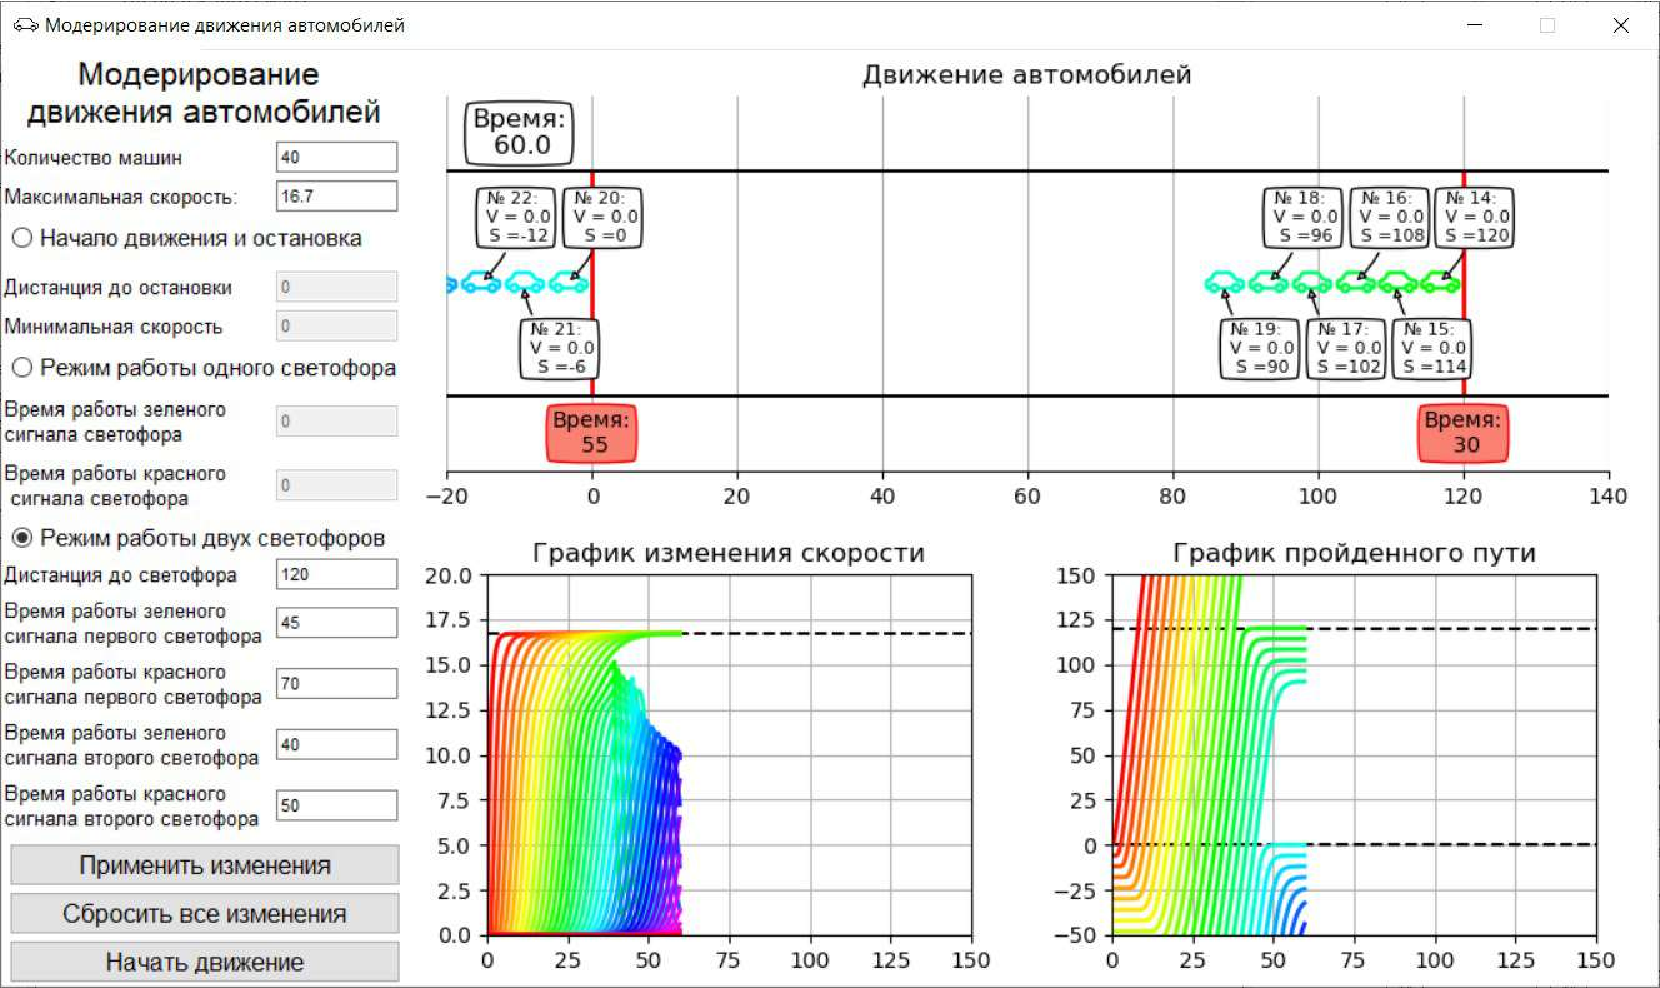
\includegraphics[width=1\linewidth]
			{Images/screens/third_mode_4}
			\caption{Положение автомобилей через 60 секунд после начала движения.}
			\label{third_mode_4}
		\end{minipage}
		\hfill
		\begin{minipage}[h]{0.48\linewidth}
			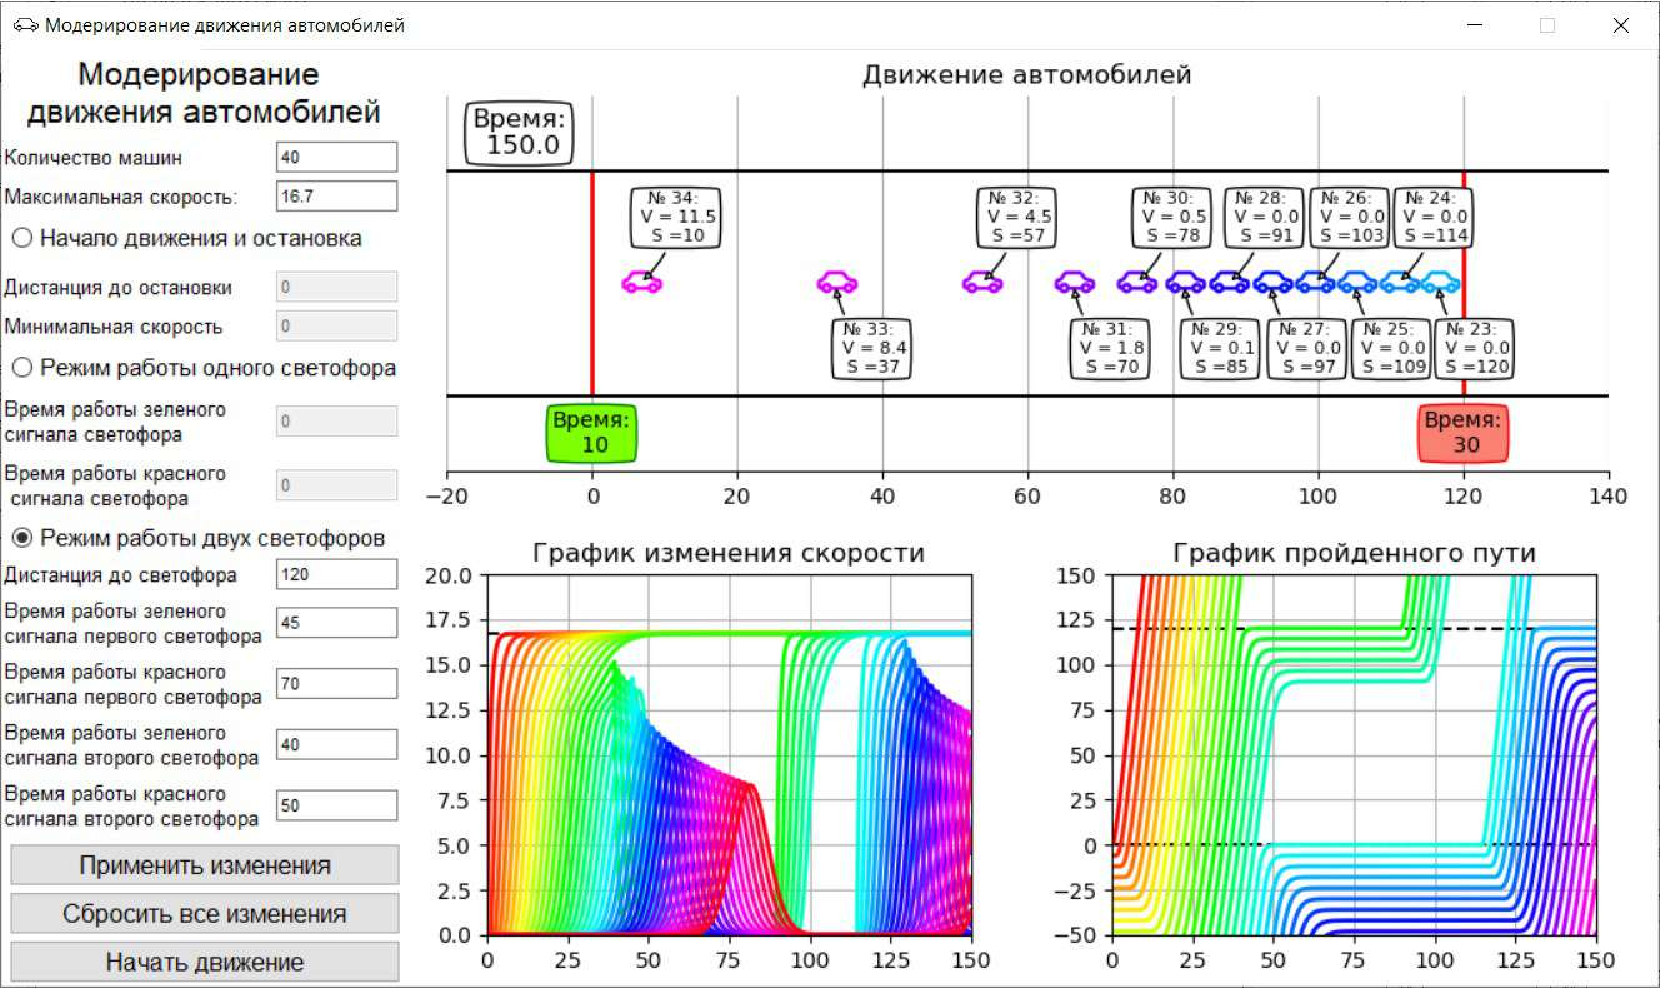
\includegraphics[width=1\linewidth]
			{Images/screens/third_mode_11}
			\caption{Положение автомобилей через 150 секунд после начала движения.}
			\label{third_mode_11}
		\end{minipage}
		\hfill 
		\begin{minipage}[h]{0.48\linewidth}
			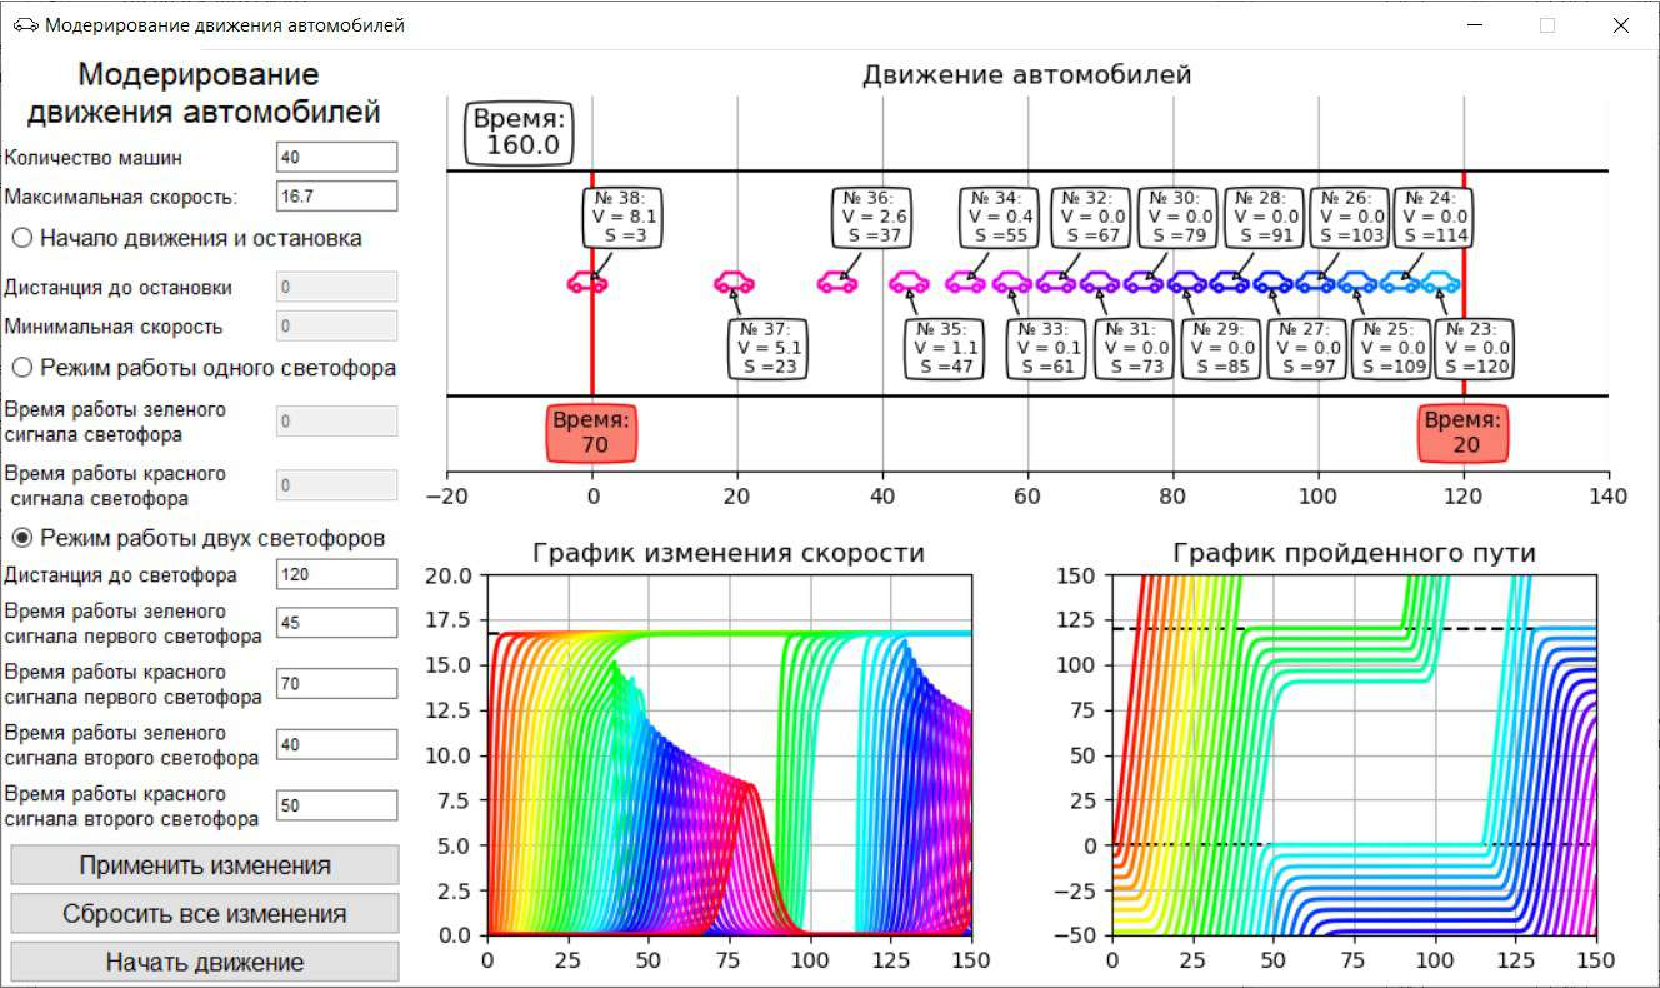
\includegraphics[width=1\linewidth]
			{Images/screens/third_mode_12}
			\caption{Положение автомобилей через 160 секунд после начала движения.}
			\label{third_mode_12}
		\end{minipage}
		\hfill 
		\begin{minipage}[h]{0.48\linewidth}
			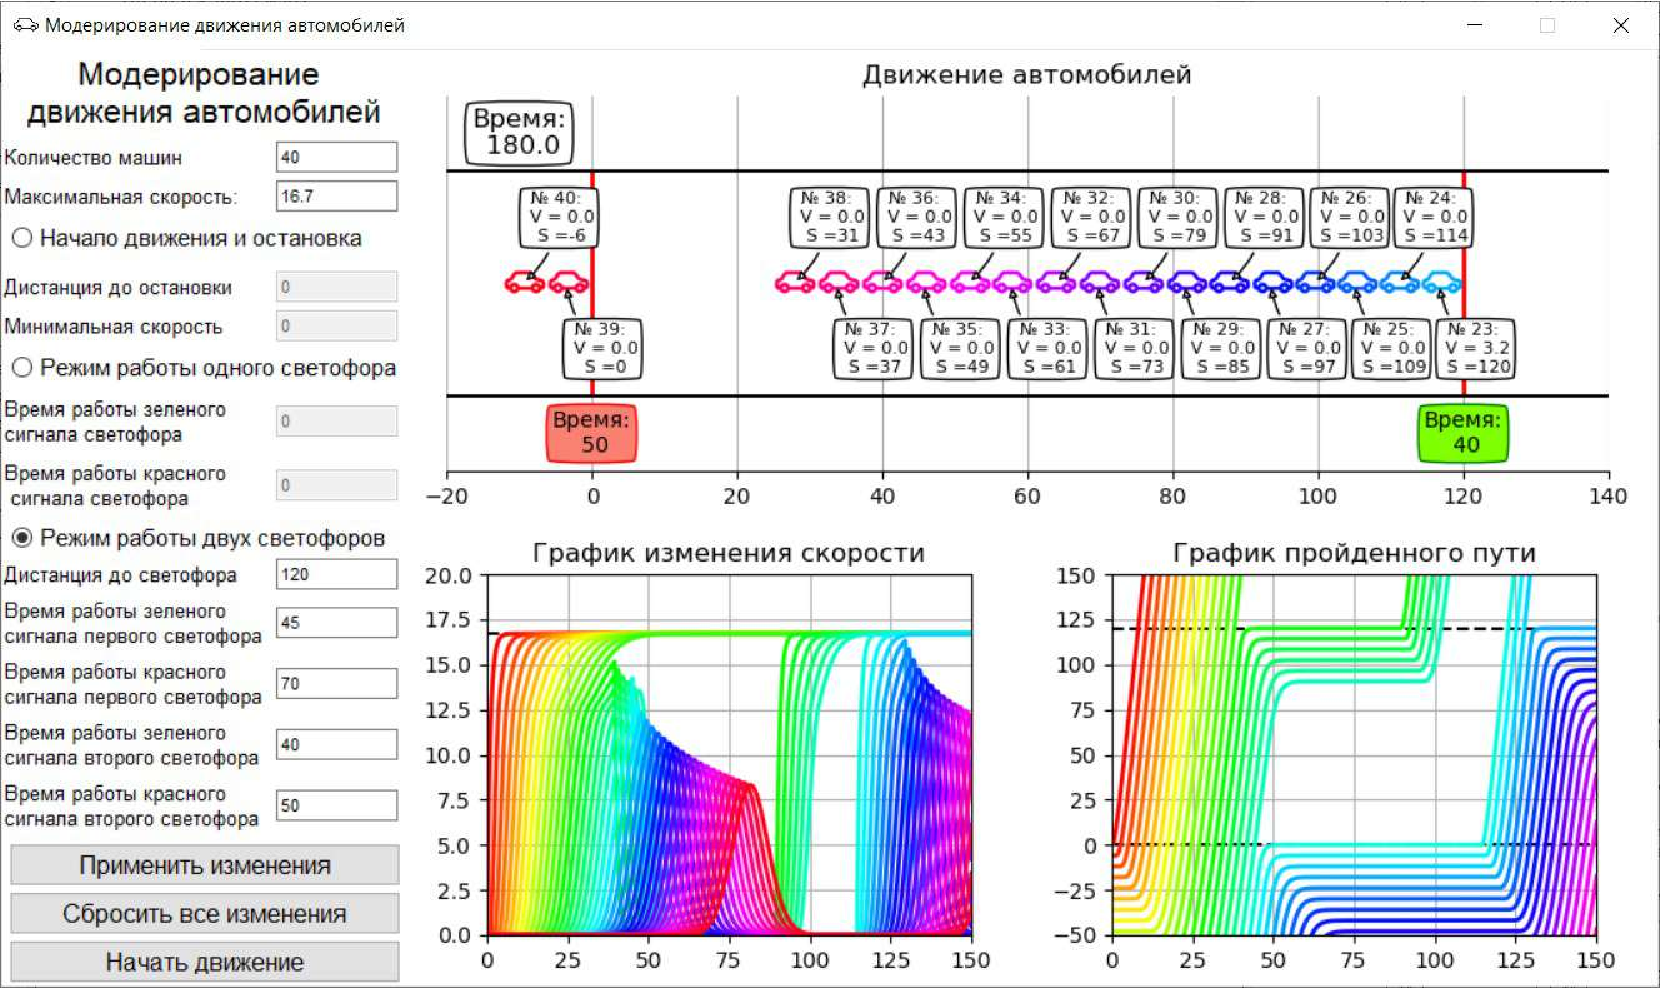
\includegraphics[width=1\linewidth]
			{Images/screens/third_mode_14}
			\caption{Положение автомобилей через 180 секунд после начала движения.}
			\label{third_mode_14}
		\end{minipage}
		\hfill 
		\begin{minipage}[h]{0.48\linewidth}
			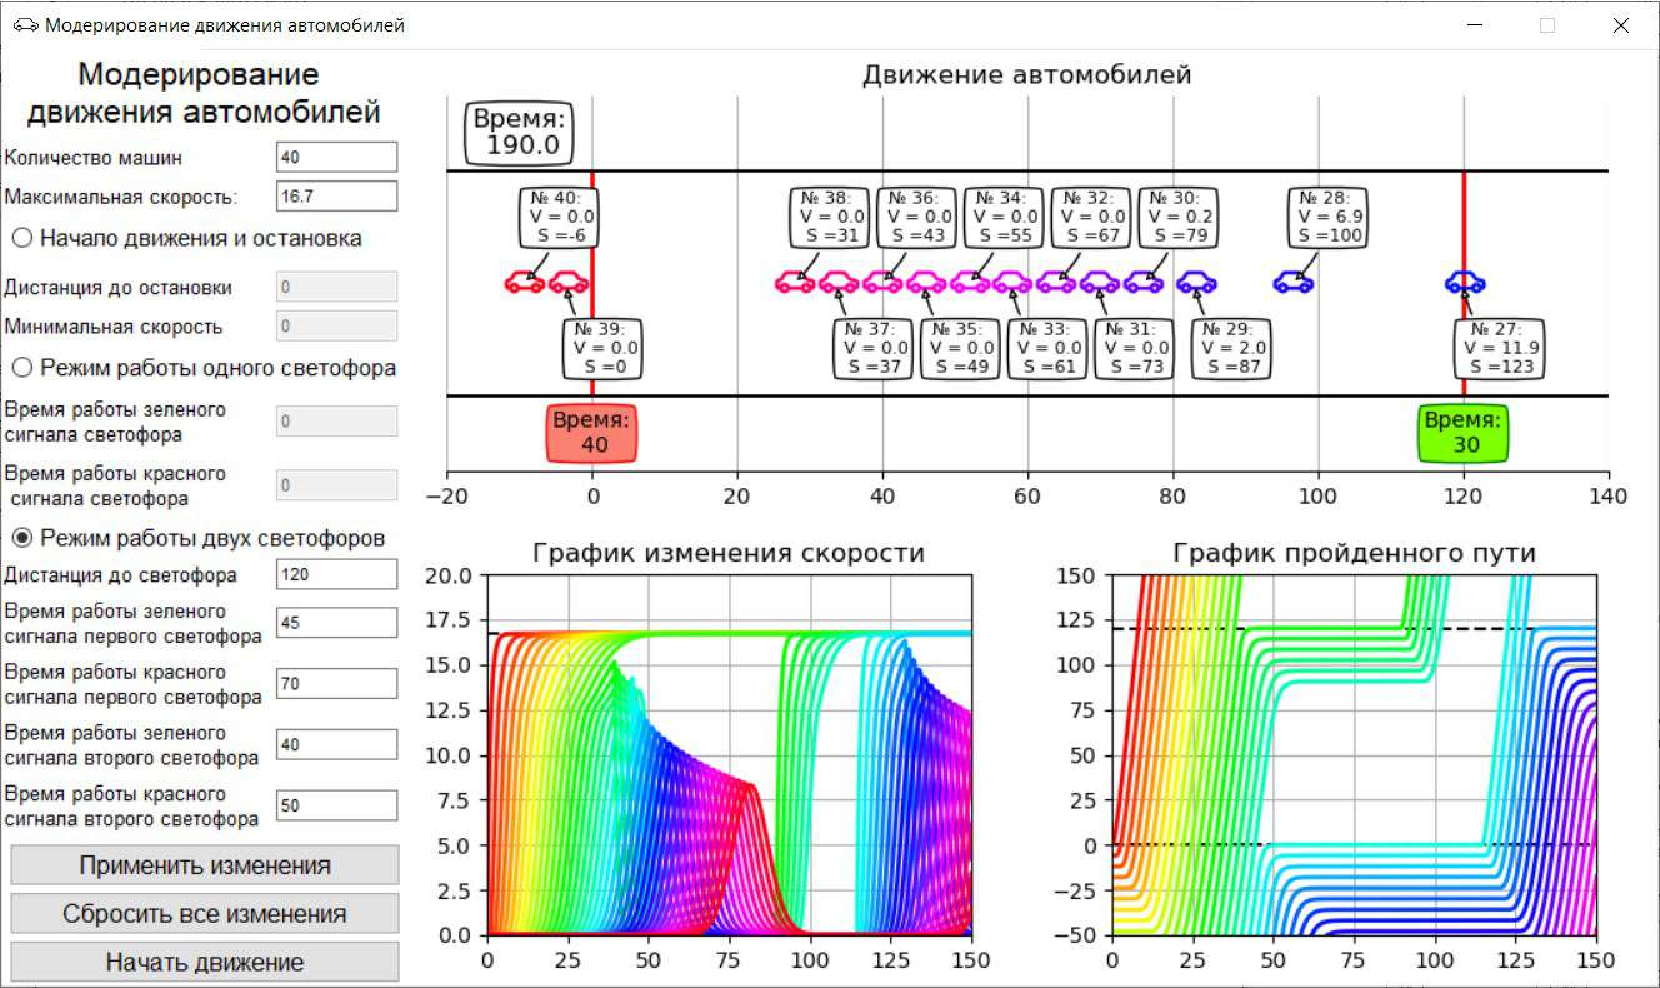
\includegraphics[width=1\linewidth]
			{Images/screens/third_mode_15}
			\caption{Положение автомобилей через 190 секунд после начала движения.}
			\label{third_mode_15}
		\end{minipage}
	\end{center}
\end{figure}

На рисунках \ref{third_mode_1}, \ref{third_mode_2}, \ref{third_mode_3}, \ref{third_mode_4}, \ref{third_mode_11} \ref{third_mode_12} \ref{third_mode_14} и \ref{third_mode_15} показано моделирование нескольких циклов работы двух реальных светофоров. Как видно из рисунков, количество автомобилей, которое проезжает через оба светофора в разработанном приложении равно среднему количеству автомобилей, который проезжают через оба реальных светофора. Это ещё раз подтверждает корректность модели \eqref{my_model}, и правильность подобранных параметров (таблица \ref{real_parameters}).

Данный режим работы программы подойдёт для моделирования участков дорог с несколькими идущими друг за другом светофорами. Данный режим программы позволяет отрегулировать режим работы каждого светофора, исключив возникновение заторов и простоев, которые могли бы возникнуть при неудачной настройке реального светофора.  

Таким образом, разработанная программа может упростить настройку светофоров, которая сейчас производится дорожными службами, преимущественно, экспериментальным путём. Экспериментальное регулирование приводит к множеству проблем, так как удачно отрегулировать режим работы светофора с первого раза можно не всегда. Это часто приводит к серьёзным последствиям, таким как пробки и заторы, а в некоторых случая и дорожно транспортные прошествия. С помощью программы можно заранее смоделировать движение транспортных потоков, посмотреть и изучить их динамику, а затем применить полученные результаты в реальной жизни.

\newpage
\section*{Заключение}
\addcontentsline{toc}{section}{Заключение}
Исходя из проведённых исследований, можно сделать вывод, что построение математической модели  движения транспортного потока нетривиальная задача и несмотря на значительный прогресс, полное понимание природы автомобильных проблем ещё не достигнуто. 

В ходе работы были рассмотрены уже существующие математические модели движения транспортных потоков, основанные на принципе следования за лидером: ``Простая модель следования за лидером''  \eqref{follow_the_leader_full_model}, ``Модель следования за лидером Дженерал моторс''  \eqref{full_gazis_model} и ``Модель разумного водителя'' \eqref{full_treiber_model_with_first_car}. Так как все эти модели обладают рядом недостатков и могут использоваться для моделирования лишь частично, то была разработана новая модель движения транспортных потоков \eqref{my_model}. 

Также в ходе работы была написана программа, которая, используя новую модель \eqref{my_model}, служит для визуализации движения автомобилей в потоке. Работа программы демонстрирует, что новая модель согласуется с динамикой реального транспортного потока.

Полученная работа позволит сделать технологии управления дорожным движением более современными, так как с помощью модели \eqref{my_model} и программы, основанной на ней, можно заранее смоделировать движение транспортного потока, а затем применить полученные результаты в реальной жизни.
\newpage

\begin{thebibliography}{**}
	\bibitem{Street}
	Дубелиръ Г.Д. ``Городскiя улицы и мостовыя''. 1912.
	
	\bibitem{TrafficFlow}
	https://spravochnick.ru/logistika/logisticheskie\_potoki/transportnyy\_potok/
	
	\bibitem{GippsModel}
	Wilson R. E. Gipps’ Model of Highway Traffic. 2002.
	
	\bibitem{WolframMathematica}
	https://www.wolfram.com
	
	\bibitem{FirstFollowTheLeaderModel}
	Pipes L.A. An operational analysis of traffic dynamics. 1953. 
	
	\bibitem{Shvetsov}
	Швецов В. И. Математическое моделирование транспортных потоков. 2003. 
	
	\bibitem{RefineFirstFollowTheLeaderModel}
	Chandler R.E., Herman R., Montroll E.W. Traffic dynamics: Studies in car following. 1958.
	
	\bibitem{Course}
	Погребняк М.А. Курсовая работа по теме ``Математическое моделирование движения транспортных потоков''. 2019.
	
	\bibitem{GazisModel}
	Gazis D.C., Herman R., Rothery R.W. Nonlinear follow the leader models of traffic flow. 1961.
	
	\bibitem{StudyingGazisModel_1}
	May, Jr. A.D., Kel ler H.E.M. Non-integer car-following models. 1967.
	
	\bibitem{StudyingGazisModel_2}
	K\"{u}hne R.D., R\"{o}diger M.B. Maсrosopiс simulation model for freeway traffic with jams
	and stop-start waves. 1991.
	
	\bibitem{StudyingGazisModel_3}
	K\"{u}hne R.D., Kroen A. Knowledge-based optimization of line сontrol systems for freeways. 1992.

	\bibitem{TreiberModel_1}
	Treiber M., Helbing D. Explanation of observed features of self-organization in traffic flow.
	1999.
	
	\bibitem{TreiberModel_2}
	Treiber M., Hennecke A., Helbing D. Congested traffic states in empirical observations and
	microscopic simulations. 2000.
	
	\bibitem{Heaviside_function}
	Земсков Ю. В. Основы теории сигналов и систем. 2003.
	
	\bibitem{PDD}
	Постановление Правительства РФ от 23.10.1993 N 1090 (ред. от 21.12.2019) "О Правилах дорожного движения" (вместе с "Основными положениями по допуску транспортных средств к эксплуатации и обязанности должностных лиц по обеспечению безопасности дорожного движения")

	\bibitem{Physics}
	Лазарев Д. А. Совершенствование дорожно-транспортной экспертизы на основе исследования процесса торможения. 2018.

	\bibitem{Python}	
	https://www.python.org
	
	\bibitem{Matplotlib}	
	https://matplotlib.org
	
	\bibitem{Runge_Kutta}
	Бахвалов Н.С.  Численные методы. 1975. 

\end{thebibliography}

\newpage

\begin{attachment} \label{att}
	\addcontentsline{toc}{section}{Приложние A}
	\begin{center}
		\vspace{1cm}
		\rm{\Large{\textbf{ Наблюдаемые характеристики работы \\ реальных светофоров }}}
		\vspace{\baselineskip}
	\end{center}

\textup{\textbf{Характеристики светофора, расположенного в городе Ярославль на перекрёстке Ленинградского проспекта и улицы Бабича }}
\newline

\noindent\textup{Расстояние до следующего светофора на перекрёстке Ленинградского проспекта и улицы Волгоградской:}

Расстояние до следующего светофора: 120 метров.

\noindent\textup{Время работы сигналов светофора:}

Время работы зелёного сигнала: 45 секунд.
			
Время работы красного сигнала: 70 секунд.

\noindent\textup{Количество автомобилей, проезжающих через светофор по одной полосе за один цикл работы:}
	
\begin{table}[h!]
	\begin{minipage}{0.23\linewidth}
		
		\centering
		\begin{tabular}{|c|c|}
			\hline
			 & Количество \\ 
			 \raisebox{1.5ex}[0cm]{№}
			 & машин 
			\\\hline
			1 & 21
			\\\hline
			2 & 16
			\\\hline
			3 & 22
			\\\hline
			4 & 18
			\\\hline
			5 & 17
			\\\hline
			6 & 19
			\\\hline
			7 & 22
			\\\hline
			8 & 22
			\\\hline
			9 & 18
			\\\hline
			10 & 16
			\\\hline
		\end{tabular}
	\end{minipage}
	\begin{minipage}{0.23\linewidth}
		\centering
		
		\begin{tabular}{|c|c|}
			\hline
			& Количество \\ 
			\raisebox{1.5ex}[0cm]{№}
			& машин  
			\\\hline
			11 & 16
			\\\hline
			12 & 15
			\\\hline
			13 & 18
			\\\hline
			14 & 21
			\\\hline
			15 & 17
			\\\hline
			16 & 15
			\\\hline
			17 & 16
			\\\hline
			18 & 25
			\\\hline
			19 & 19
			\\\hline
			20 & 18
			\\\hline
		\end{tabular}
	\end{minipage} 
	\begin{minipage}{0.23\linewidth}
		\centering
	
		\begin{tabular}{|c|c|}
			\hline
			& Количество \\ 
			\raisebox{1.5ex}[0cm]{№}
			& машин 
			\\\hline
			21 & 21
			\\\hline
			22 & 20
			\\\hline
			23 & 18
			\\\hline
			24 & 13
			\\\hline
			25 & 15
			\\\hline
			26 & 20
			\\\hline
			27 & 20
			\\\hline
			28 & 22
			\\\hline
			29 & 28
			\\\hline
			30 & 21
			\\\hline
		\end{tabular}
	\end{minipage} 
	\begin{minipage}{0.23\linewidth}
		\centering
	
		\begin{tabular}{|c|c|}
			\hline
			& Количество \\ 
			\raisebox{1.5ex}[0cm]{№}
			& машин 
			\\\hline
			31 & 15
			\\\hline
			32 & 17
			\\\hline
			33 & 19
			\\\hline
			34 & 18
			\\\hline
			35 & 18
			\\\hline
			36 & 14
			\\\hline
			37 & 26
			\\\hline
			38 & 19
			\\\hline
			39 & 20
			\\\hline
			40 & 16
			\\\hline
		\end{tabular}
	\end{minipage}
\end{table}

\noindent Среднее количество автомобилей, проезжающих через светофор: 18.775 $\approx$ 19.
\newline

\noindent\textup{Данные характеристики были собраны в период с 01.03.2020 по 01.05.2020 }.
\newpage

\textup{\textbf{Характеристики светофора, расположенного в городе Ярославль на перекрёстке Ленинградского проспекта и улицы Волгоградской }}
\newline

\noindent\textup{Расстояние до предыдущего светофора на перекрёстке Ленинградского проспекта и улицы Бабича:}

Расстояние до предыдущего светофора: 120 метров.

\noindent\textup{Время работы сигналов светофора:}

Время работы зелёного сигнала: 40 секунд.

Время работы красного сигнала: 50 секунд.

\noindent\textup{Количество автомобилей, проезжающих через светофор по одной полосе за один цикл работы:}

\begin{table}[h!]
	\begin{minipage}{0.23\linewidth}
		
		\centering
		\begin{tabular}{|c|c|}
			\hline
			& Количество \\ 
			\raisebox{1.5ex}[0cm]{№}
			& машин 
			\\\hline
			1 & 16
			\\\hline
			2 & 10
			\\\hline
			3 & 15
			\\\hline
			4 & 12
			\\\hline
			5 & 8
			\\\hline
			6 & 11
			\\\hline
			7 & 13
			\\\hline
			8 & 10
			\\\hline
			9 & 12
			\\\hline
			10 & 12
			\\\hline
		\end{tabular}
	\end{minipage}
	\begin{minipage}{0.23\linewidth}
		\centering
		
		\begin{tabular}{|c|c|}
			\hline
			& Количество \\ 
			\raisebox{1.5ex}[0cm]{№}
			& машин  
			\\\hline
			11 & 16
			\\\hline
			12 & 11
			\\\hline
			13 & 15
			\\\hline
			14 & 10
			\\\hline
			15 & 11
			\\\hline
			16 & 13
			\\\hline
			17 & 18
			\\\hline
			18 & 10
			\\\hline
			19 & 10
			\\\hline
			20 & 11
			\\\hline
		\end{tabular}
	\end{minipage} 
	\begin{minipage}{0.23\linewidth}
		\centering
		
		\begin{tabular}{|c|c|}
			\hline
			& Количество \\ 
			\raisebox{1.5ex}[0cm]{№}
			& машин 
			\\\hline
			21 & 9
			\\\hline
			22 & 12
			\\\hline
			23 & 11
			\\\hline
			24 & 13
			\\\hline
			25 & 14
			\\\hline
			26 & 11
			\\\hline
			27 & 10
			\\\hline
			28 & 13
			\\\hline
			29 & 13
			\\\hline
			30 & 13
			\\\hline
		\end{tabular}
	\end{minipage} 
	\begin{minipage}{0.23\linewidth}
		\centering
		
		\begin{tabular}{|c|c|}
			\hline
			& Количество \\ 
			\raisebox{1.5ex}[0cm]{№}
			& машин 
			\\\hline
			31 & 8
			\\\hline
			32 & 10
			\\\hline
			33 & 11
			\\\hline
			34 & 10
			\\\hline
			35 & 12
			\\\hline
			36 & 19
			\\\hline
			37 & 16
			\\\hline
			38 & 14
			\\\hline
			39 & 11
			\\\hline
			40 & 12
			\\\hline
		\end{tabular}
	\end{minipage}
\end{table}
\noindent Среднее количество автомобилей, проезжающих через светофор: 12.15 $\approx$ 12.
\newline

\noindent\textup{Данные характеристики были собраны в период с 01.03.2020 по 01.05.2020 }.
\end{attachment}


\newpage

\begin{attachment} \label{att2}
	\addcontentsline{toc}{section}{Приложние B}
	\begin{center}
		\vspace{1cm}
		\rm{\Large{\textbf{ Диск \\ с исходным кодом программы }}}
		\vspace{\baselineskip}
	\end{center}
\end{attachment}
\end{document}